\documentclass[]{article}

% include packages needed for your report
\usepackage{graphicx, verbatim, qtree} % to include figures
\usepackage{caption,subcaption} % to include captions and sub captions to figures
\usepackage{titling} % to format title page
\renewcommand\maketitlehooka{\null\mbox{}\vfill} % to center title page
\renewcommand\maketitlehookd{\vfill\null}
\usepackage[margin=1.1in]{geometry} % to adjust the page margin
\usepackage{amsmath} % to display equations
\usepackage{csquotes} % to quote
\usepackage{float} % specify figure and table location
\usepackage{fancyhdr} % to add header
\usepackage{lastpage} % to put the current page number in context of page numbers in the whole document
\usepackage[nottoc,numbib]{tocbibind} % to give section number for the reference
\usepackage{enumitem} % to adjust spacing between bullet point and dashed line
\usepackage{longtable}

\pagestyle{fancy}
\fancyhf{}
\cfoot{Page \thepage \hspace{0.9pt} of \pageref{LastPage}}

\rhead{AS}
\lhead{
\includegraphics[scale=0.02]{uclalogo.png}}

\title{\Huge Prostate Cancer Active Surveillance }
\date{\today}
\author{\\[1cm]
      Author Alfonso Lam\\[1.5cm]
      Boutros Lab\\
      Jonsson Comprehensive Cancer Center\\
      }

% begin report
\begin{document}

% title page
\begin{titlingpage}
\maketitle
\begin{figure}
    \centering
    
\includegraphics[scale=0.03]{uclalogo.png}
    \label{fig:my_label}
\end{figure}
\end{titlingpage}

% The idea here is that patients with prostate cancer often go on
% something called “Active Surveillance” (AS). This means that they
% have the disease, but the chance of it becoming aggressive and moving
% outside of the prostate is very low (~5-10%).
%
% Because this chance is low, patients will often be “surveilled” to
% see if their disease advances
% using a combination of blood tests, imaging and biopsies. The current
% prediction of “is this cancer aggressive” is not perfect, and in
% fact biopsy is an aggressive & expensive procedure.  There is therefore
% a need to do a better job in making these predictions.
% 
% Our colleague in San Antonio, Dr. Michael Liss, is a prostate cancer
% surgeon (i.e. a urologist) and has accumulated a cohort of 123 patients
% who were on AS a fraction of which went on to aggressive disease
% (the “Biopsy Upgraded” column in the
% MRI DOD Biomarkers Database_Boutros – 2019.11.12.xlsx).
% He then did a series of imaging, genetic, blood and urine tests on
% these patients to try to predict aggressive disease.
% 
% The questions we have in this dataset are two-fold:
% 
% 1.- What features best predict aggressive disease?
% 
% 2.- In what order (sequence) should different biomarkers be run
% to maximize sensitivity and specificity, while minimizing cost?
% Note here that the word “sequence” in this study can both refer to the
% technology used to analyze genetic information on patients
% (“they were sequenced” or “sequencing data”) and to the ordering of different
% tests (“what sequence should these tests be run?”) and it will be critical
% that you are extremely clear in writing which of these two you’re
% referring to at all times.
% 
% As you’ll see there are a couple of files labeled –Key which explain
% the individual features.  As with the m6A-writer dataset you will want
% to start with exploratory analysis (EDA – exploratory data analysis):
% 
% Look at distributions
% Look at correlations amongst variables
% Create some plots outlining the dataset as a whole
% 
% Then you’ll move on to univariate analyses
% 
% How does each predictive feature correlate to the outcome variable?
% 
% Then you’ll move on to sequencing of biomarkers.
% This will involve considering all the biomarkers that emerge from a
% single assay and asking which assay provides the most information
% as an initial test, and then which is most complementary to it, and so forth.
% We will then likely consider the “cost” (financial) of each biomarker
% as a weight in this decision making, but we can consider detailed
% strategies at a later date once we’ve seen the EDA.
% 
% As before, I want this sequentially built up into a PDF report in
% the lab format, so that at any point in time we have a report of all
% the results that have been generated to date, along with their associated
% methods.  And I’ll link you in a moment to Dr. Liss, although let me
% know before you ask him any questions directly as he’s a surgeon and
% I don’t want to take up his time with minor questions.

% report outline
\section{Introduction}

\subsection{Study Design and Objectives}
\noindent In this study, a group of individuals with prostate cancer is on
“Active Surveillance” (AS). AS is a combination of blood tests, imaging and biopsies. 
It intends to monitor the progression of the disease, but the current prediction of 
the aggressiveness of prostate cancer is not perfect and needs improvement. What features 
do the best job in predicting aggressive disease? In what order (sequence) should 
different biomarkers be run to maximize sensitivity and specificity, while minimizing cost?  

\subsection{Data Description}

\begin{center}
\begin{tabular}{ |c|p{2cm}|p{2cm}|}
\hline
  {\bf Filename} &  {\bf Number of Individuals} & {\bf Number of Columns}  \\
\hline
    MRI\_DOD\_Biomarkers\_Database\_Boutros$-$2020.04.20.xlsx &  123  & 53  \\
\hline
\end{tabular}
\end{center}

\section{Exploratory Data Analysis}

\noindent Some basic information from the individuals are available in the original dataset. 
Figure~\ref{fig:basic} shows some of the basic features the patients have. \\

\begin{figure}[H]
\centering
\begin{tabular}{|c|c|}
      \hline
      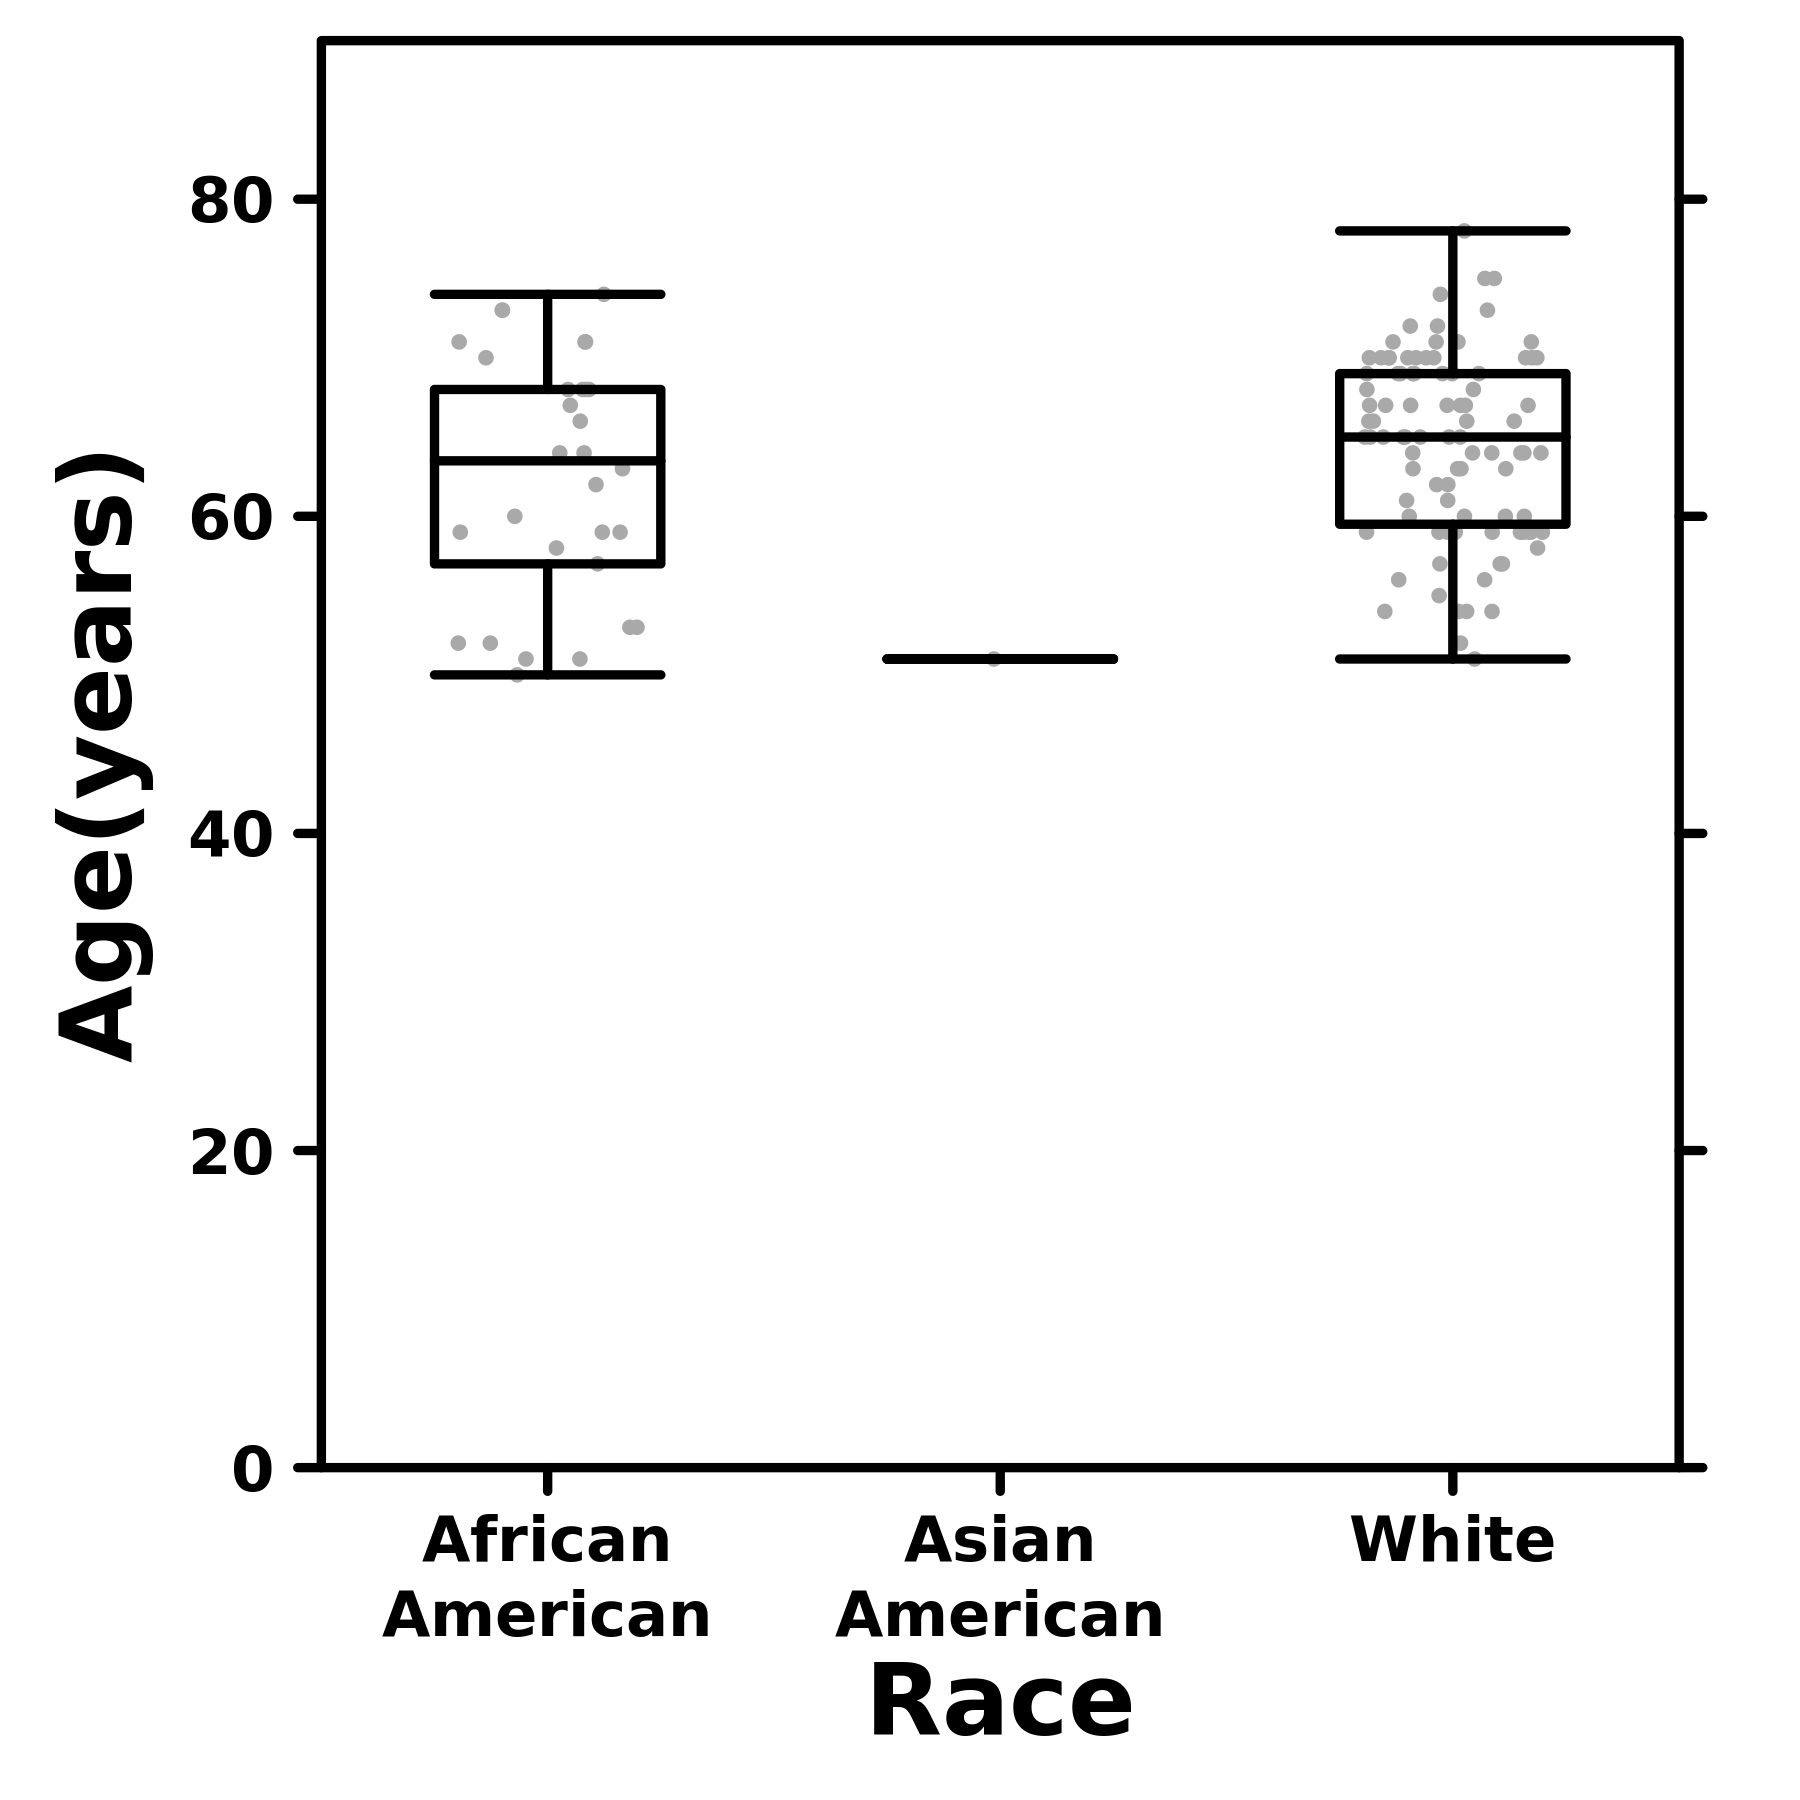
\includegraphics[width=40mm]{png/age.png} &
      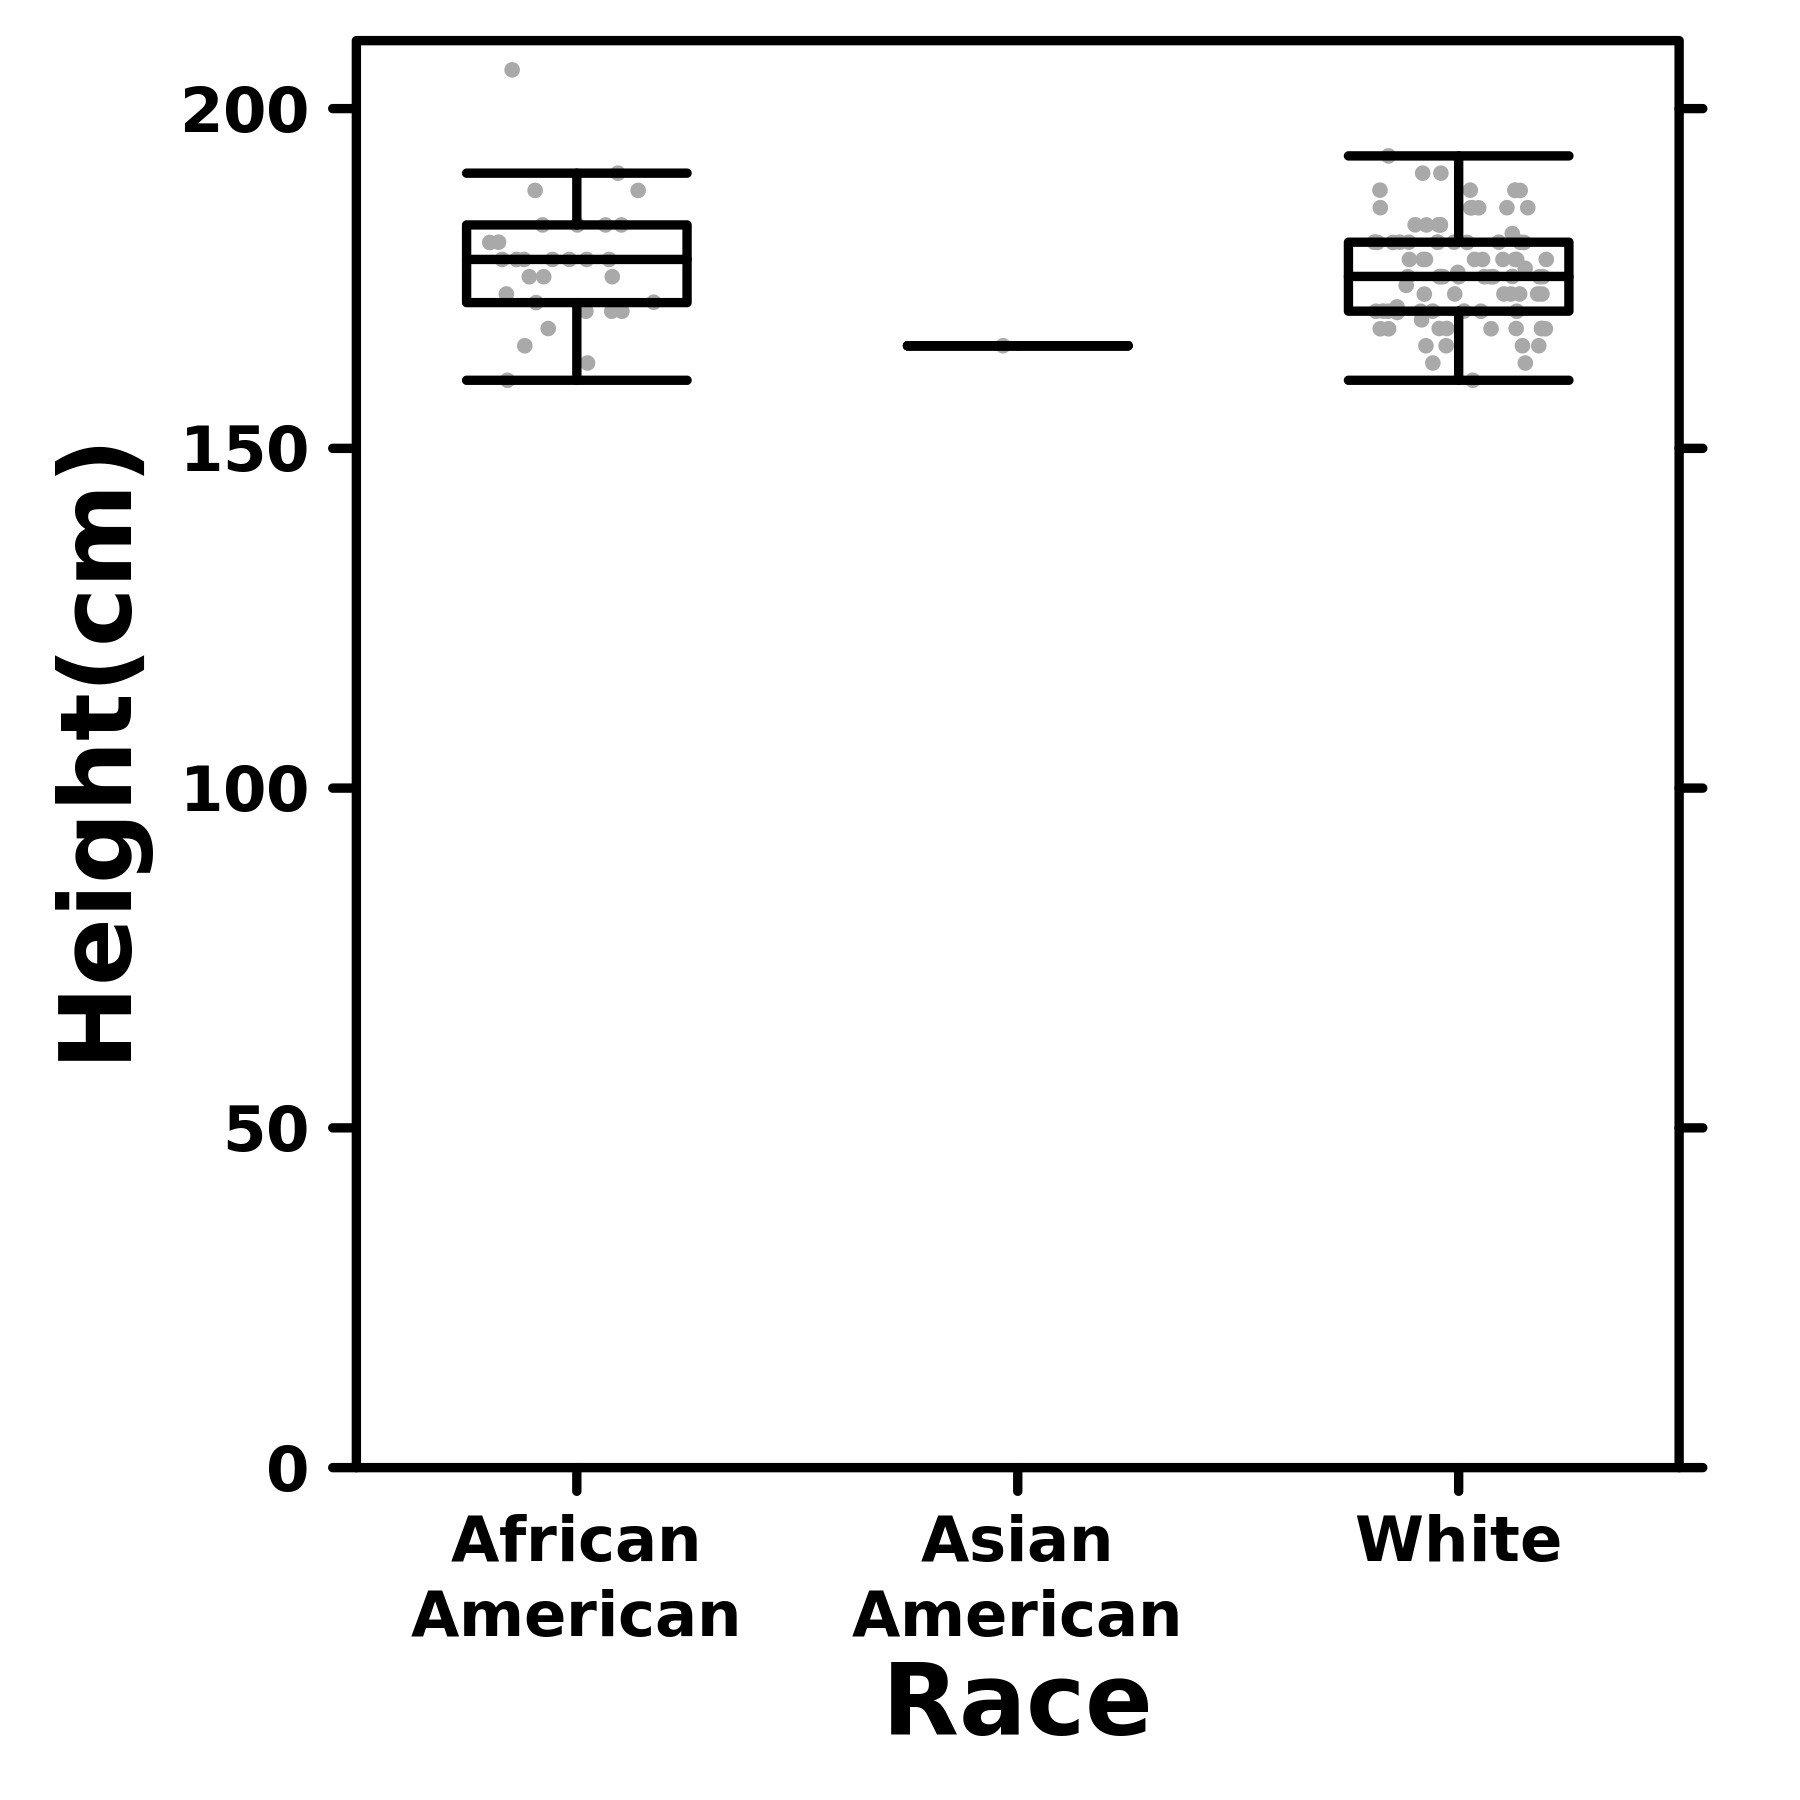
\includegraphics[width=40mm]{png/height.png} \\
      \hline
      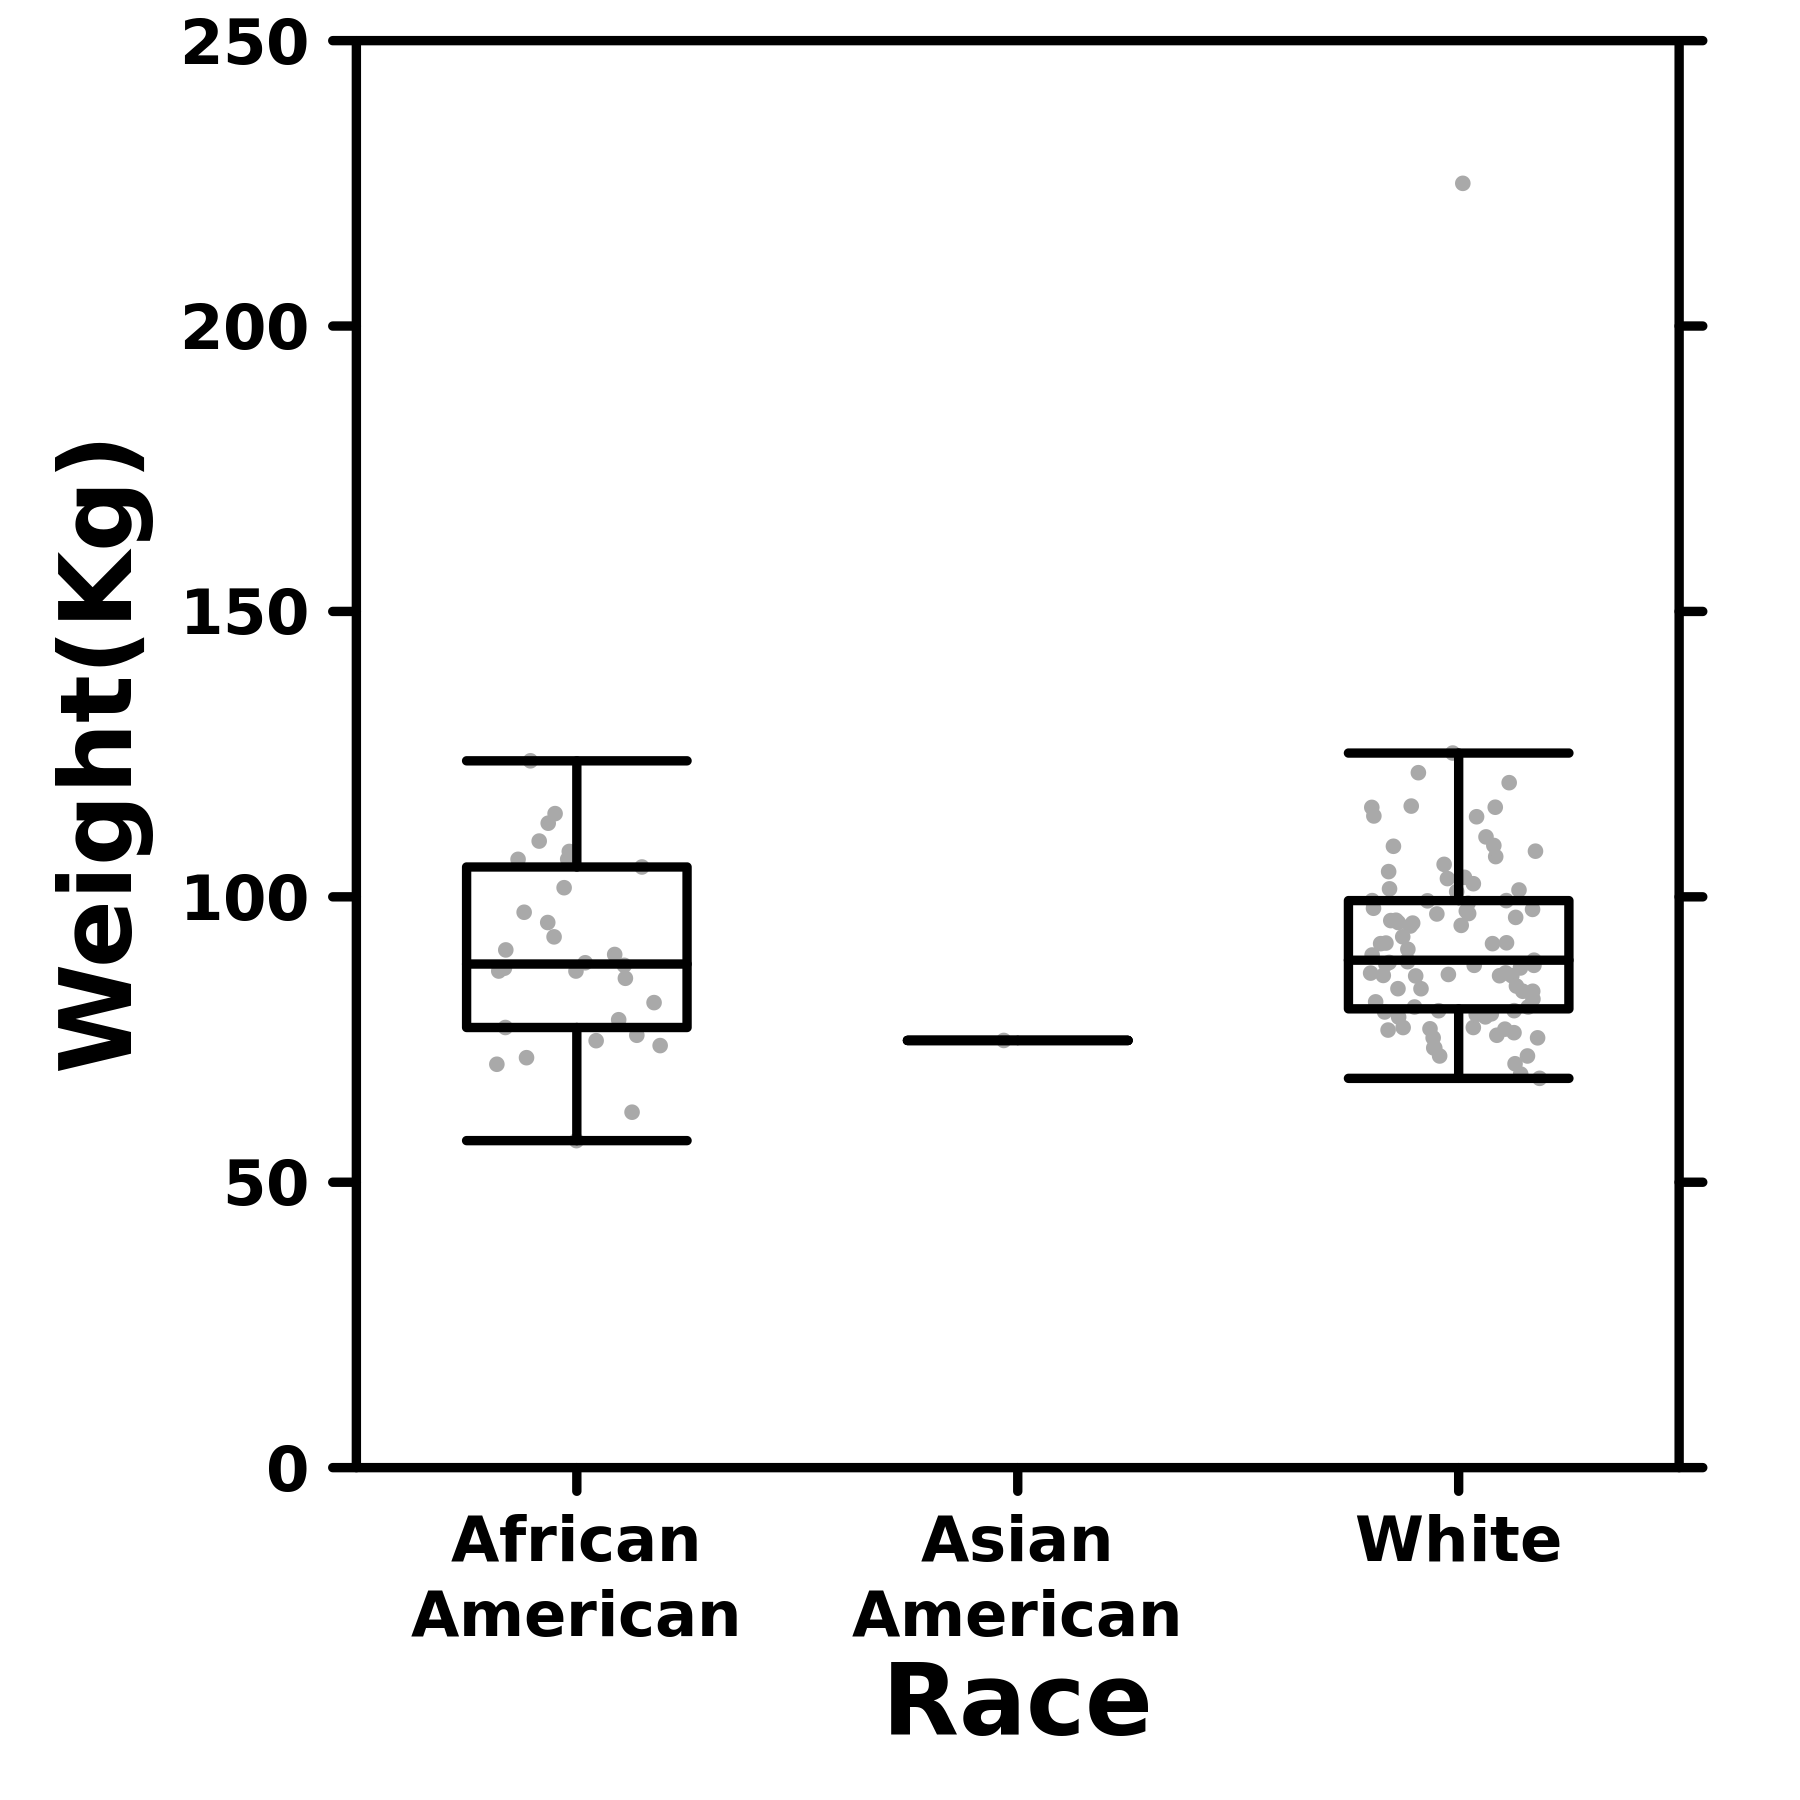
\includegraphics[width=40mm]{png/weight.png} & 
      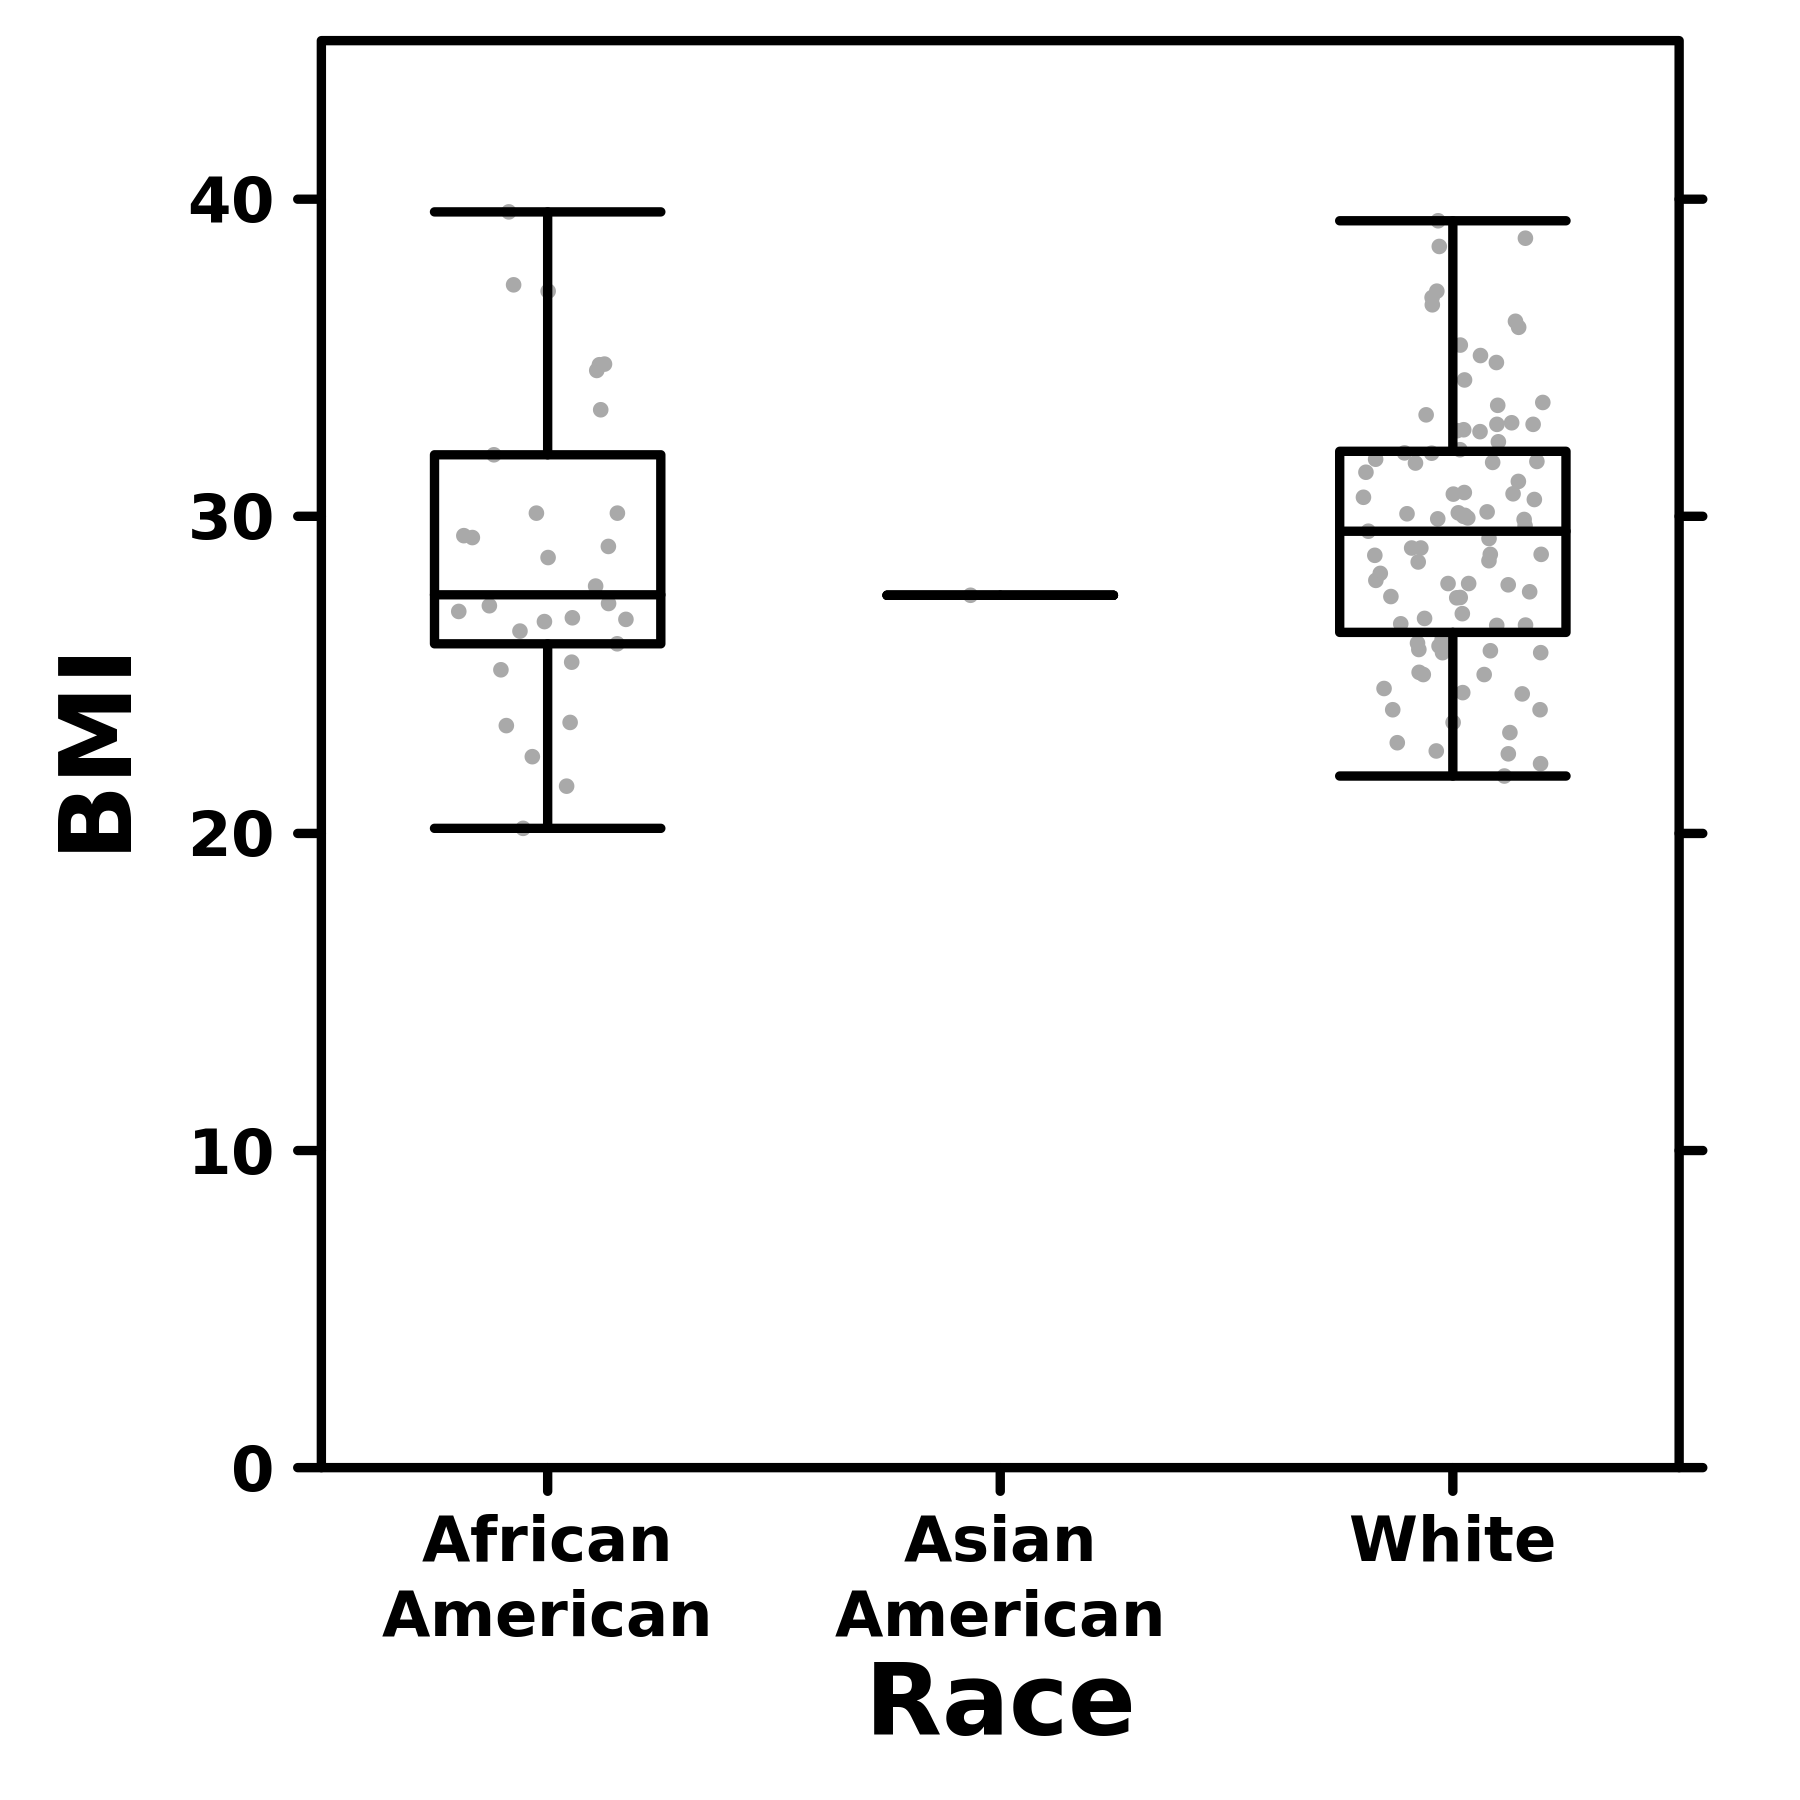
\includegraphics[width=40mm]{png/bmi.png} \\
      \hline
\end{tabular}
\caption{Basic information from individuals grouped by race: African-American, Asian-American, and White}
\label{fig:basic}
\end{figure}

\noindent Figure~\ref{fig:basic2} shows the prostate volume distributed in the individuals. These individuals 
are patients that were administered blood test, urine test, MRI, biopsies, etc. They are currently on 
AS and not all of them did all the tests.  \\

\begin{figure}
\centering
    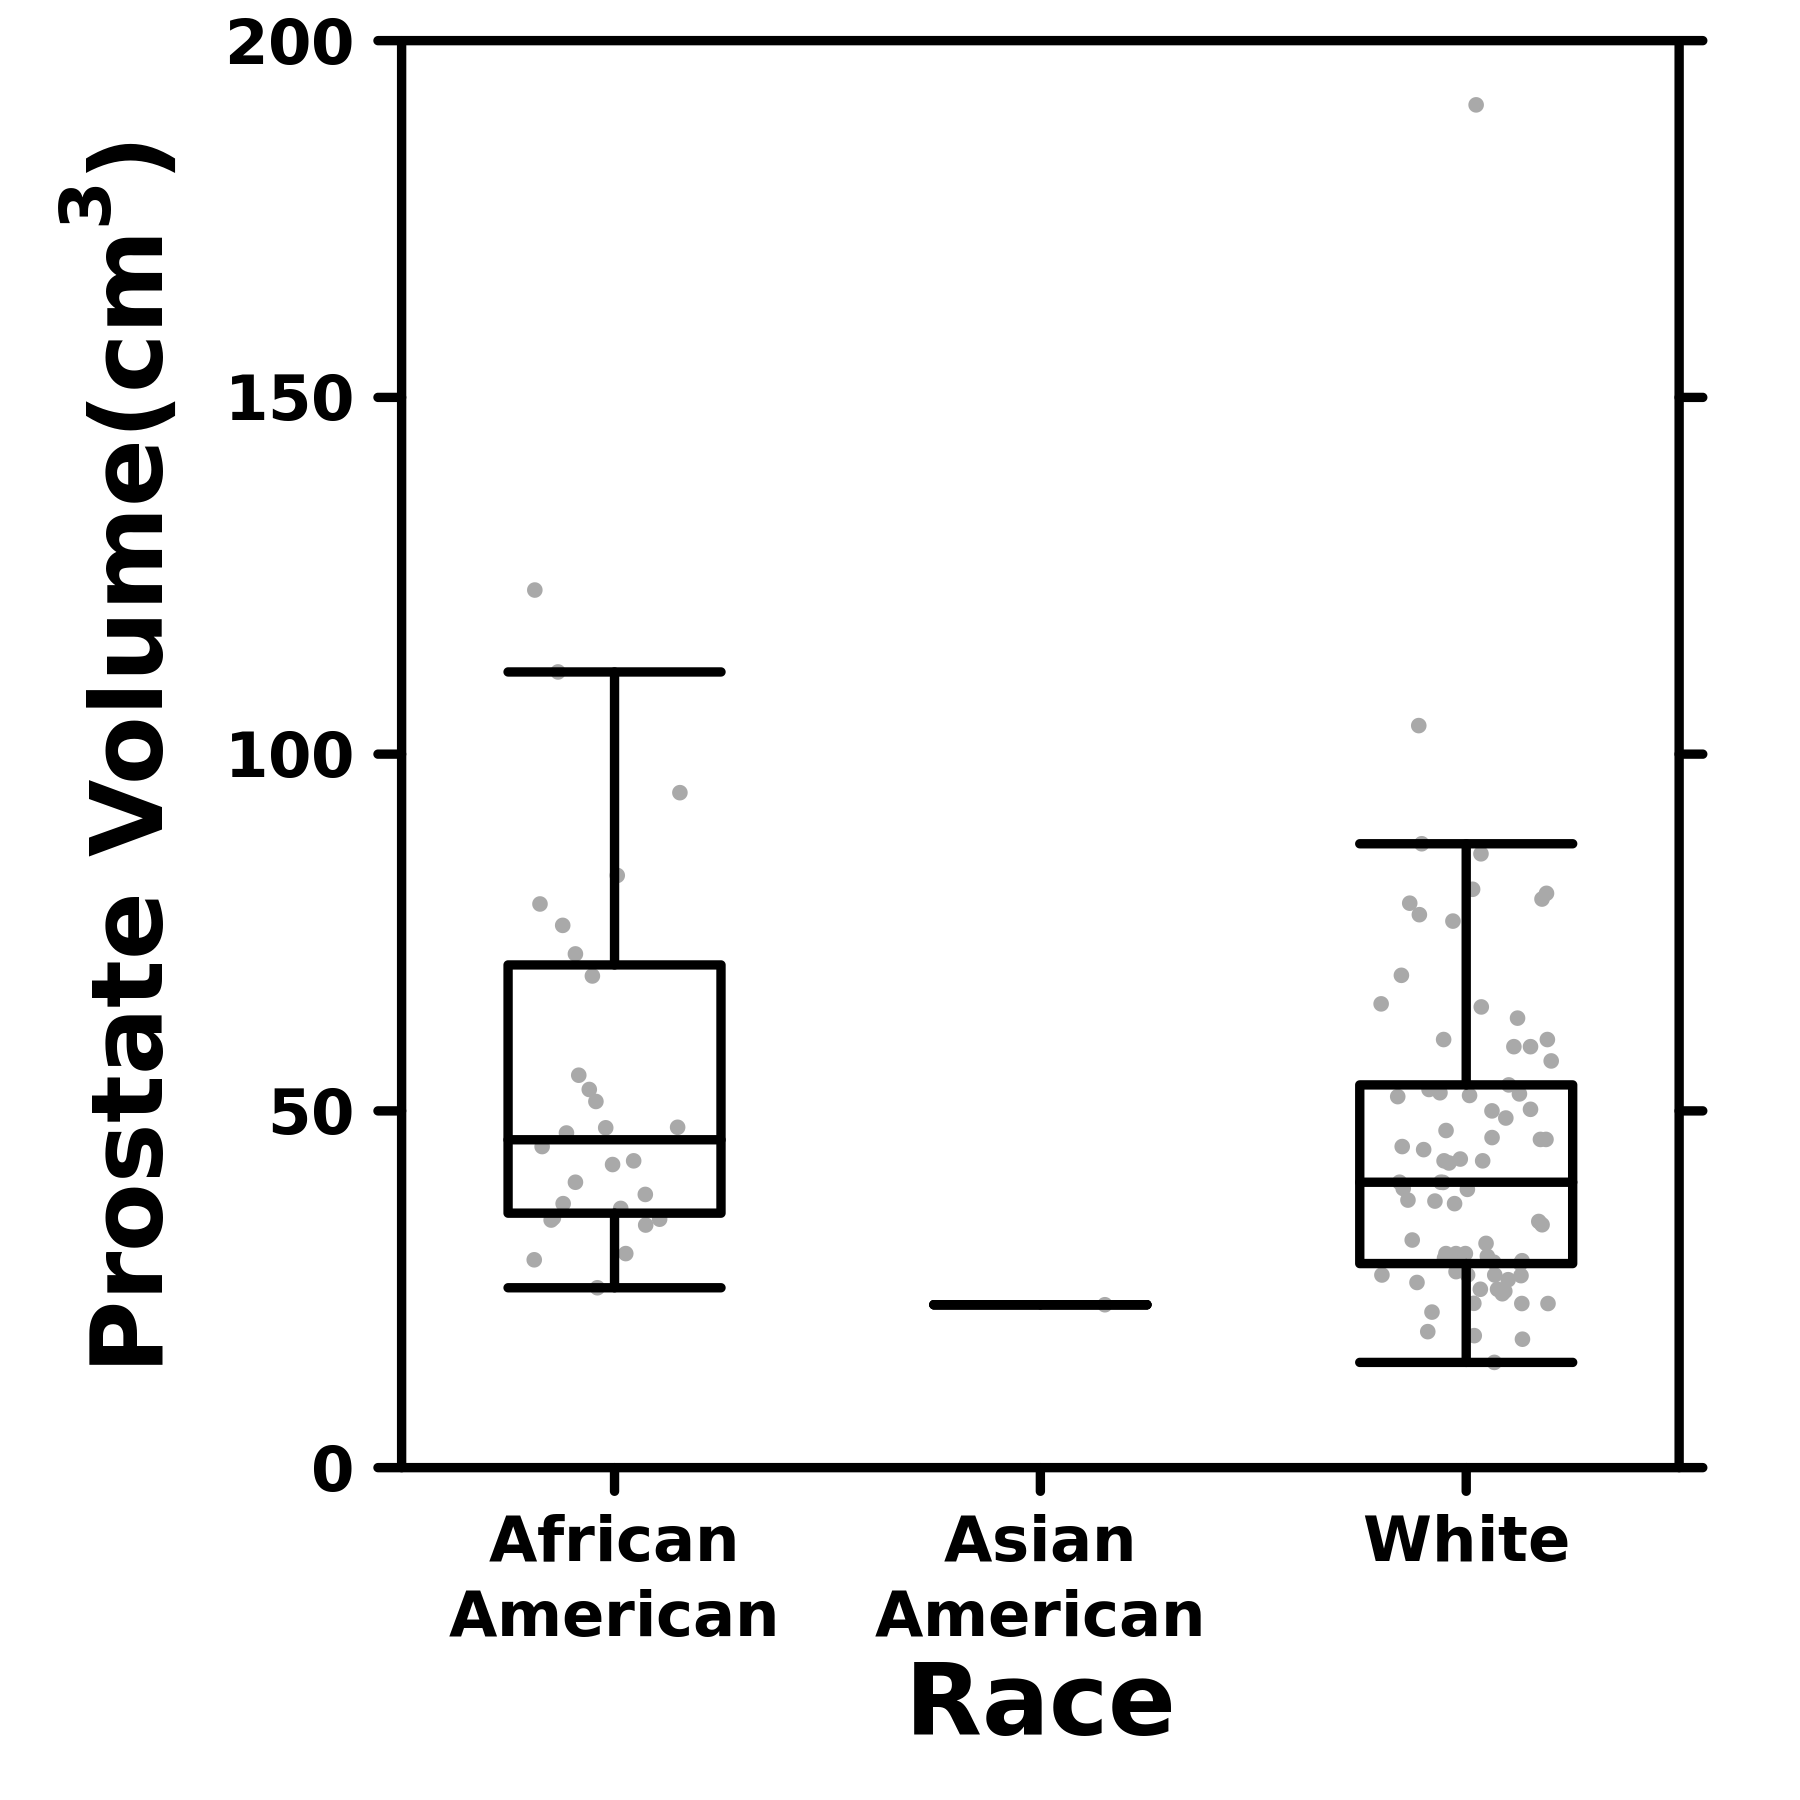
\includegraphics[width=50mm]{png/prostate_volume.png} \\
\caption{Prostate volume for the three different groups of subjects.}
\label{fig:basic2}
\end{figure}

\noindent In the original dataset, most of those tests report numerical quantities or scores, and others  
reporting binary responses (0 or 1, etc). As part of the exploratory data analysis, Table~\ref{table:summary} summarizes 
the data in the tests analyzed in this report. \\

\begin{longtable}{|c|c|p{1.5cm}|c|c|p{1.5cm}|c|} 
\hline
{\bf Test} &  {\bf Minimum}  & {\bf First Quarter} &  {\bf Median}  & {\bf Mean}  & {\bf Third Quarter}  & {\bf Maximum}   \\
\hline
      ADC normal Signal &     3.00       &  17.00       &    32.50  &  45.57  &          50.75  &     264.00  \\
\hline
      ADC lesion Signal &     0.00       &   1.00       &    18.50  &  77.09  &          64.00  &     919.00  \\
\hline
      RSI lesion Signal &    16.00       &  34.25       &    55.00  &  53.93  &          71.75  &      94.00  \\
\hline
      RSI normal Signal &     6.00       &  15.00       &    31.00  &  33.15  &          45.50  &      77.00  \\
\hline
                   PCA3 &     1.20       &   4.05       &     6.25  &   6.96  &           8.67  &      30.40  \\
\hline
                  T2ERG &     0.17       &   0.52       &     0.79  &   0.93  &           1.10  &       3.87  \\
\hline
       MiPS Cancer Risk &     1.73       &   7.73       &    12.84  &  29.05  &          19.09  &    1561.00  \\
\hline
  MiPS High Grade Cancer Risk &     3.20       &   9.70       &    13.65  &  14.96  &          17.80  &      41.30  \\
\hline
       PSA Hybrid &     5.40       &  27.60       &    36.55  &  41.63  &          54.38  &     101.20  \\
\hline
         free PSA &     1.00       &   1.00       &     1.00  &   1.55  &           2.00  &       4.00  \\
\hline
         PSA Density  & 0.003952   &  0.011972    &     0.018269  & 0.021220 & 0.025472 & 0.121317 \\
\hline
            p2PSA &     1.00       &   8.00       &    24.00  &  33.79  &          52.00  &      98.00  \\
\hline
 Percent Free PSA &     1.00       &   1.00       &     2.00  &   1.67  &           2.00  &       3.00  \\
\hline      
              PHI &     0.00       &   0.00       &     0.00  &   0.17  &           0.00  &       1.00  \\
\hline      
          PHI Density &  0.0750 &  0.5371 & 0.8927 & 1.0839 & 1.4006 & 3.8899 \\
\hline 
           SOCPSA &     0.00       &   0.00       &     0.00  &   0.19  &           0.00  &       2.00  \\
\hline
     TNFa Average &     0.00       &   0.00       &     0.00  &   0.12  &           0.00  &       1.00  \\
\hline
 Genetic Ancestry &     0.00       &   0.00       &     0.00  &   0.36  &           0.00  &       5.00  \\
\hline
 Genetic Risk Score &     0.00       &   0.00       &     0.00  &   0.07  &           0.00  &       4.00  \\
\hline
 Genetic Risk Category &     1.07       &   2.16       &     2.89  &   2.76  &           3.24  &       4.58  \\
\hline
 Global Screening Array &    23.40       & 833.11       &  1031.24  & 994.27  &        1189.62  &    1736.73  \\
\hline
   GSA Positives &    -1.53       & 495.67       &   637.40  & 650.40  &         780.48  &    1202.47  \\
\hline
   BRCA Mutation &     3.60       &  29.05       &    42.04  &  54.43  &          54.77  &     848.73  \\
\hline
   Mutation 1 &     1.50       &   8.80       &    16.98  &  17.23  &          23.57  &      41.19  \\
\hline
   Mutation 2 &     1.18       &   3.77       &     5.56  &   6.89  &           8.35  &      60.00  \\ 
\hline
\caption{Descriptive statistics of the tests administered to the subjects.}
\label{table:summary}
\end{longtable}

\noindent Some of these tests are related to other tests or are combination of simpler tests. To quantify these
relations, Spearman's correlation between tests and subjects features are computed. The result is shown 
in Figure~\ref{fig:correlations}. The information from the heatmap will be useful to reduce the number 
of tests used for the sequential testing. \\

\begin{minipage}{\linewidth}
\makebox[\linewidth]{
  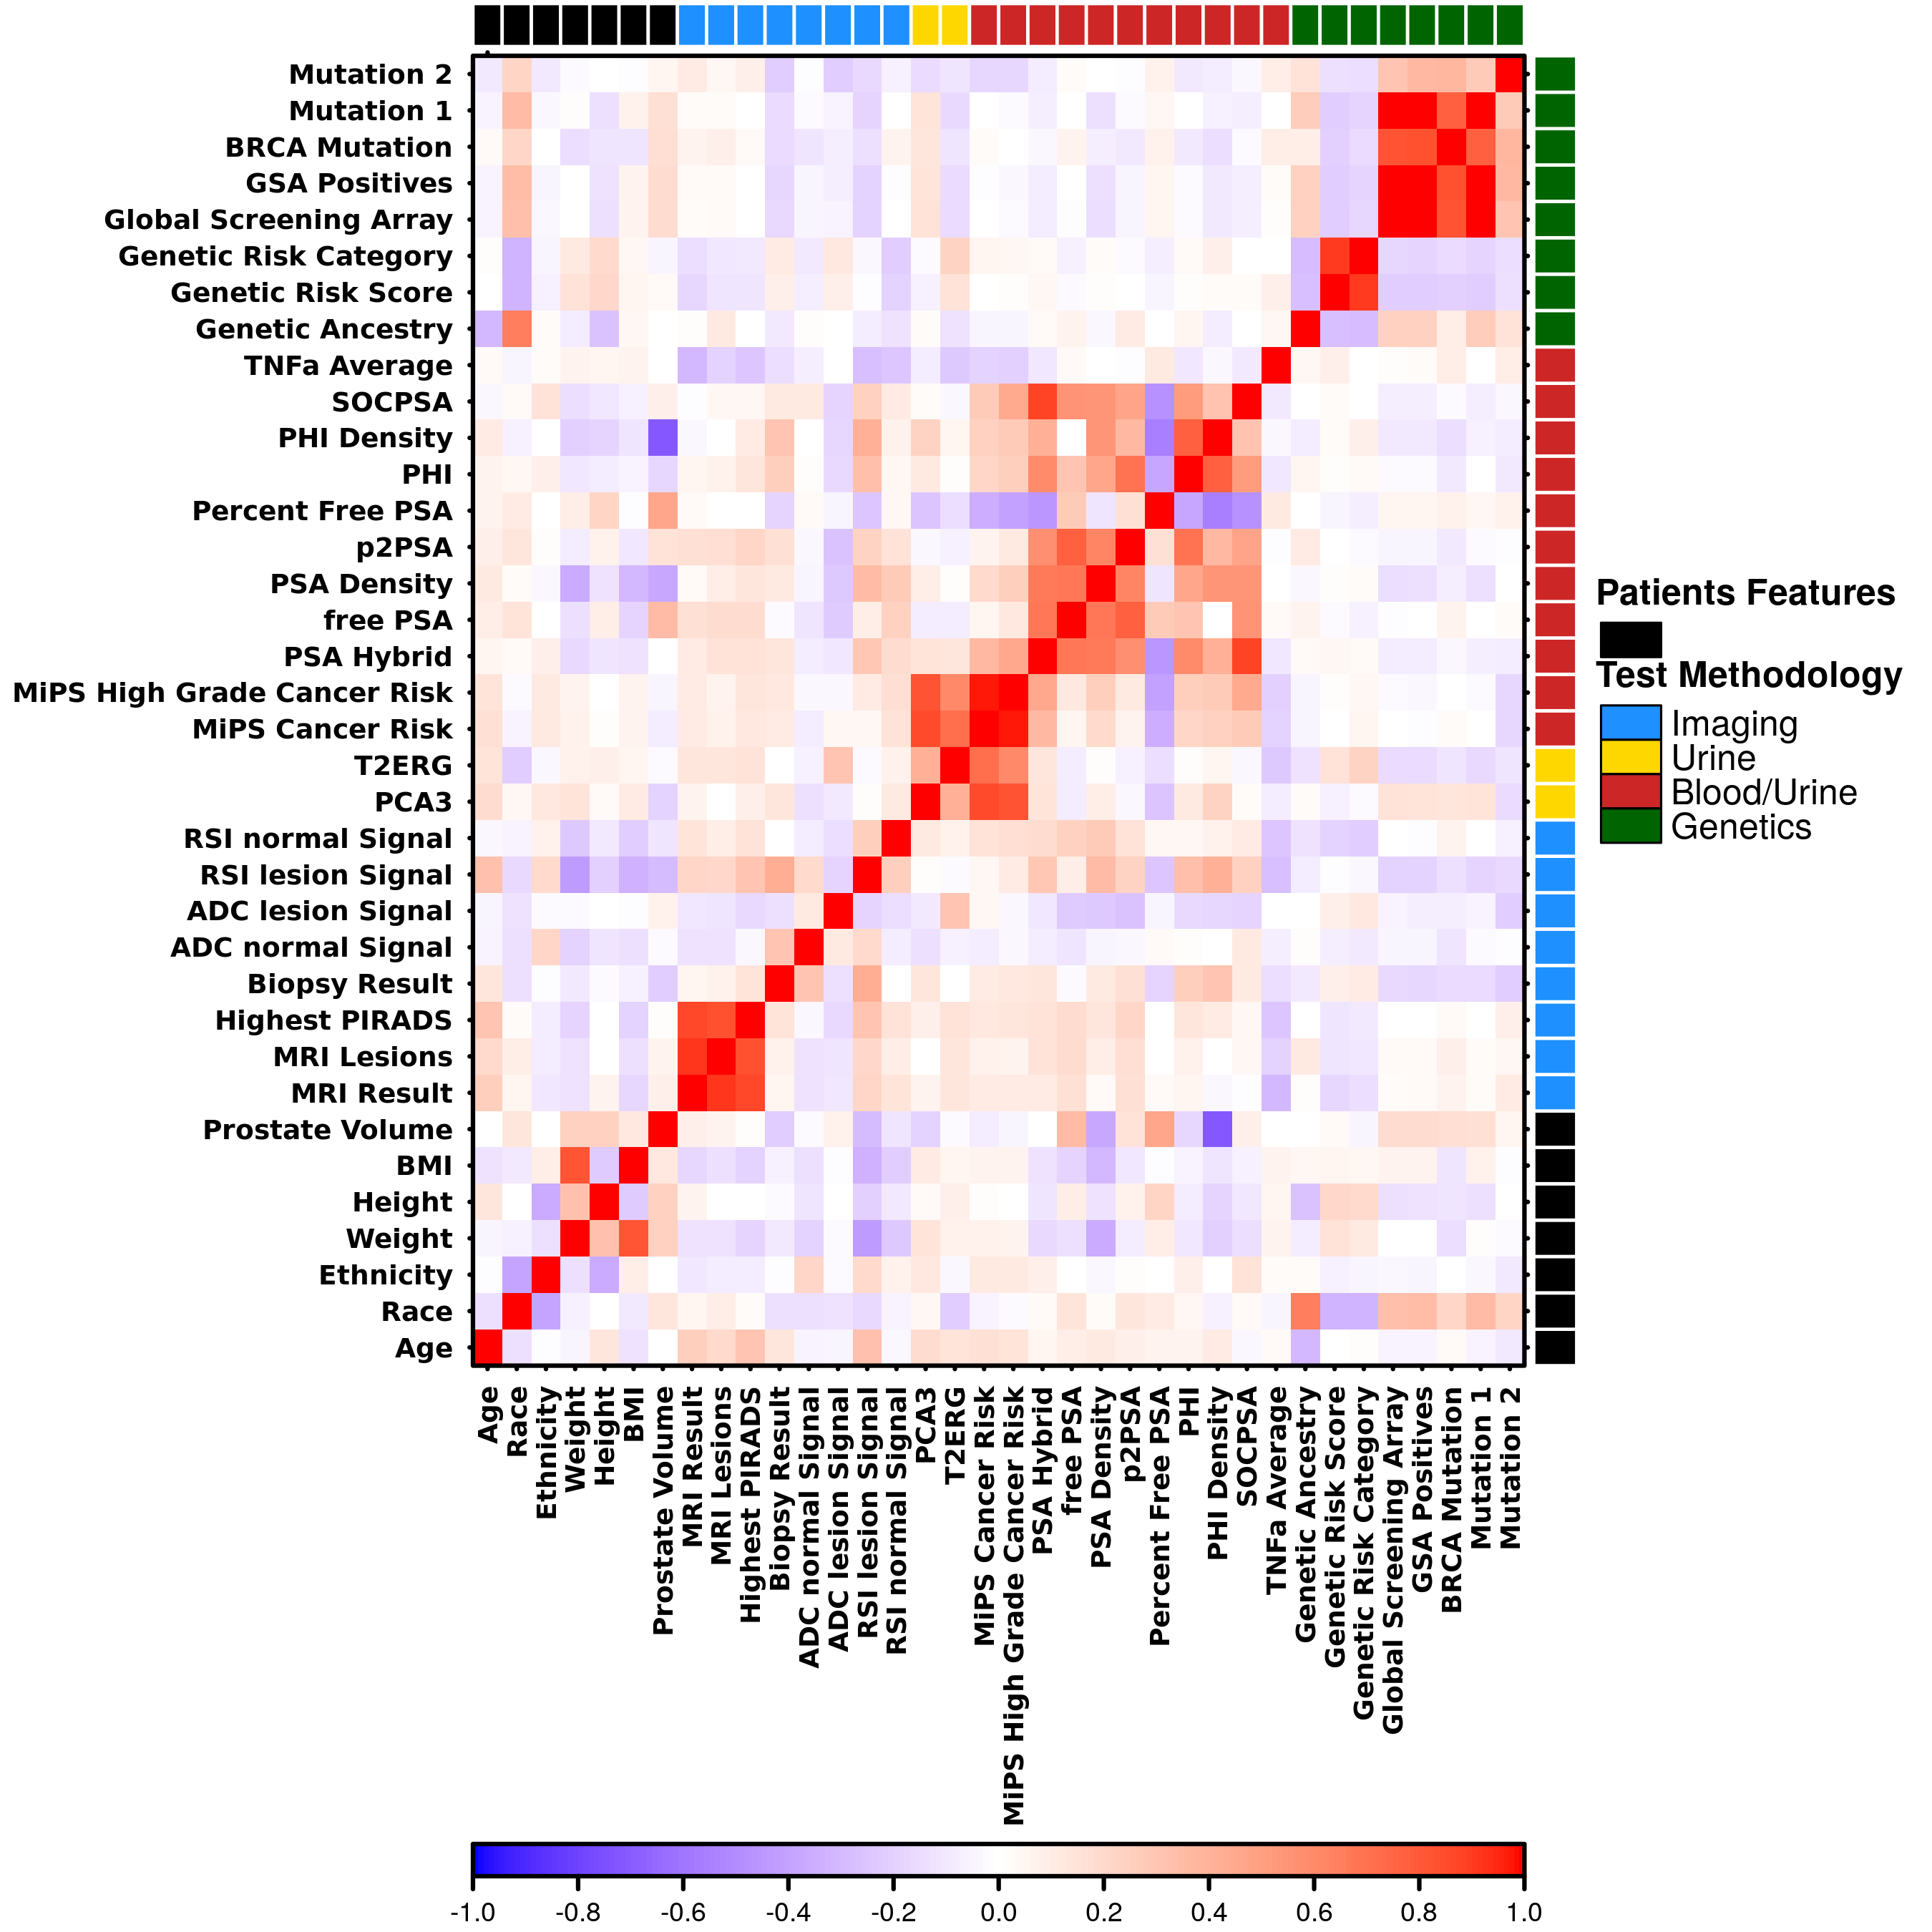
\includegraphics[keepaspectratio=false,scale=0.6]{png/correlations.png}
}
\captionof{figure}{Correlations between features of the subjects and tests performed in the subjects.}
\label{fig:correlations}     
\end{minipage} \\

\newpage

\noindent By definition, a patient on AS has prostate cancer. Thus, a sequence of tests are performed during the
AS in order to monitor the progression of the disease. At some point in time, the doctor updates the biopsy information
({\verb|BiopsyUpgraded|}). It is a categorical variable (0=No, 1=Yes) and will be used as the gold standard 
to determine a relation between the {\verb|BiopsyUpgraded|} with the different biomarkers used in the AS. 
Those biomarkers are shown in the Appendix section. \\

\noindent For each test, its performance is evaluated by plotting the Precision-Recall (PR) Curve. 
The PR curves for all the tests are displayed in Figure~\ref{fig:PRcurve}. From that figure, most of the test 
have in general low precision, except \verb|RSIlesionSignal| where particularly shows a larger area under 
the curve in comparison to other tests. Figure~\ref{fig:roc_plot} shows the ROC curves of the tests. Several of
those tests are on the diagonal line or even below, which indicates they have low or no predictive power. 
Figure~\ref{fig:auprc_auroc_plot} summarizes the areas under the curve for the PR-curves and ROC-curves.\\

\begin{minipage}{\linewidth}
\makebox[\linewidth]{
  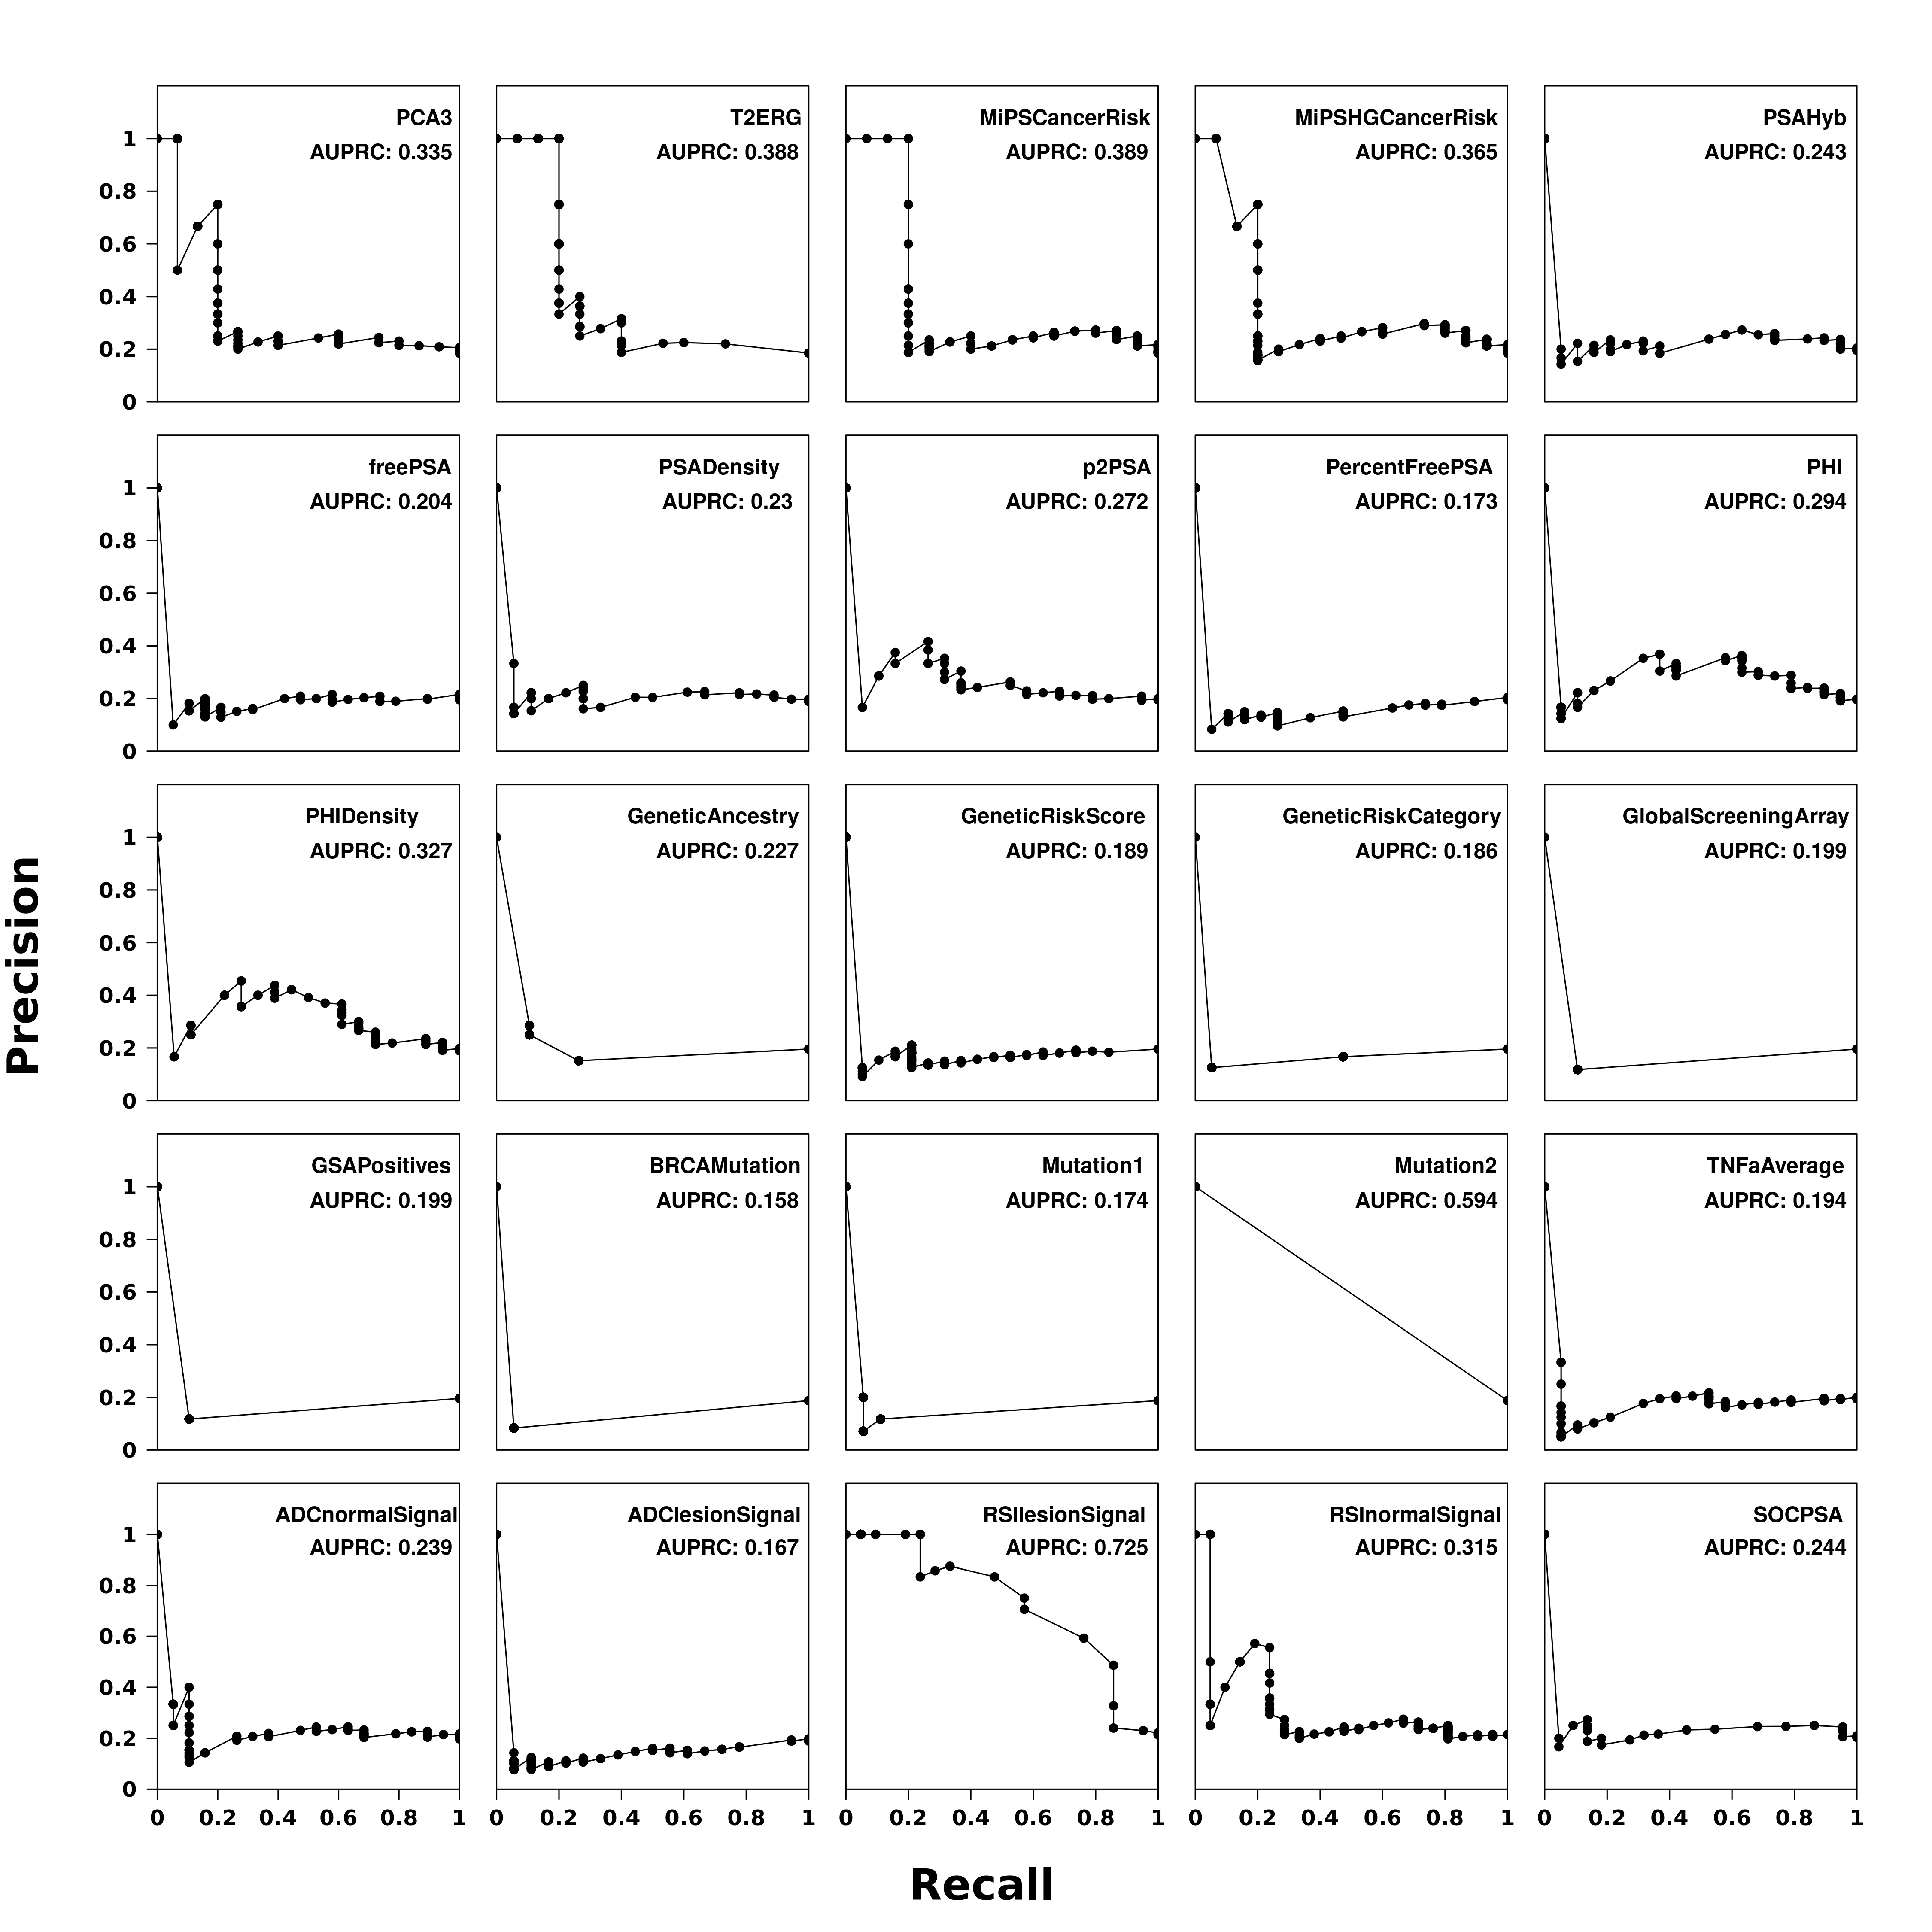
\includegraphics[keepaspectratio=false,scale=0.4]{png/multipanelplot_prc.png}
}
\captionof{figure}{Precision-Recall Curves of the tests used in AS.}
\label{fig:PRcurve}     
\end{minipage} \\

\begin{minipage}{\linewidth}
\makebox[\linewidth]{
  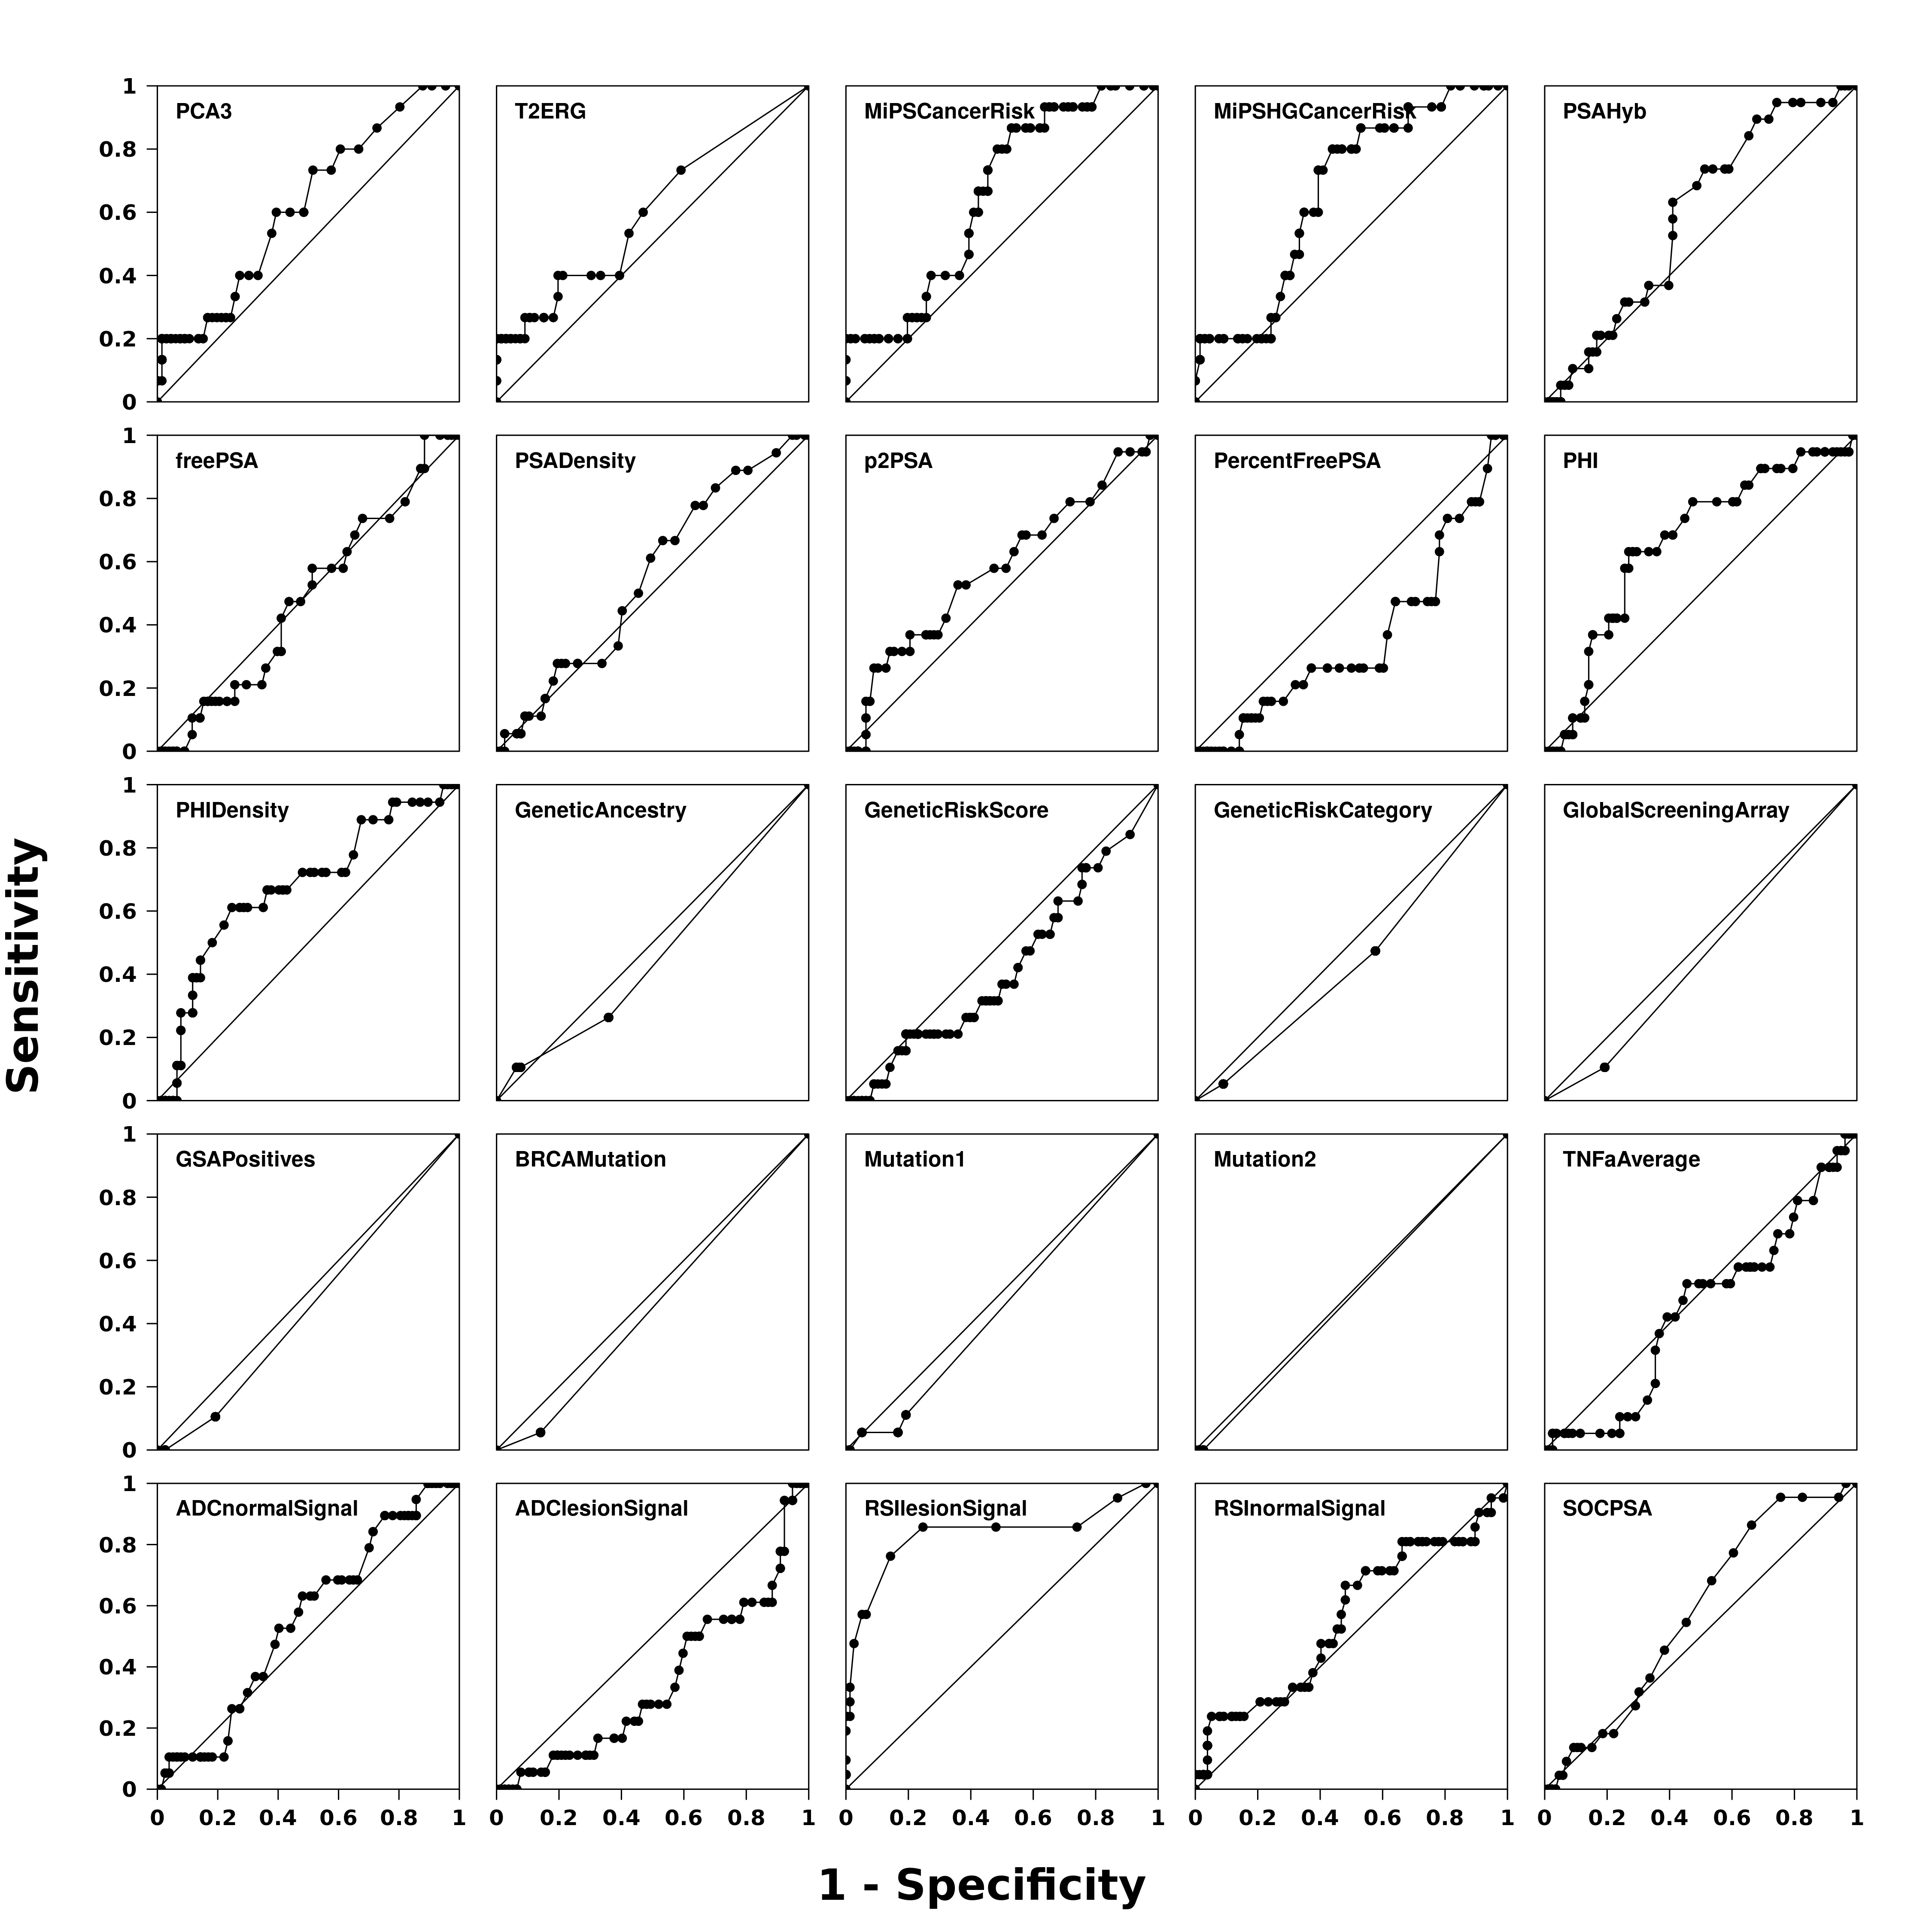
\includegraphics[keepaspectratio=false,scale=0.4]{png/multipanelploprt_roc.png}
}
\captionof{figure}{ROC Curves of the tests used in AS.}
\label{fig:roc_plot}     
\end{minipage} \\

\begin{minipage}{\linewidth}
\makebox[\linewidth]{
  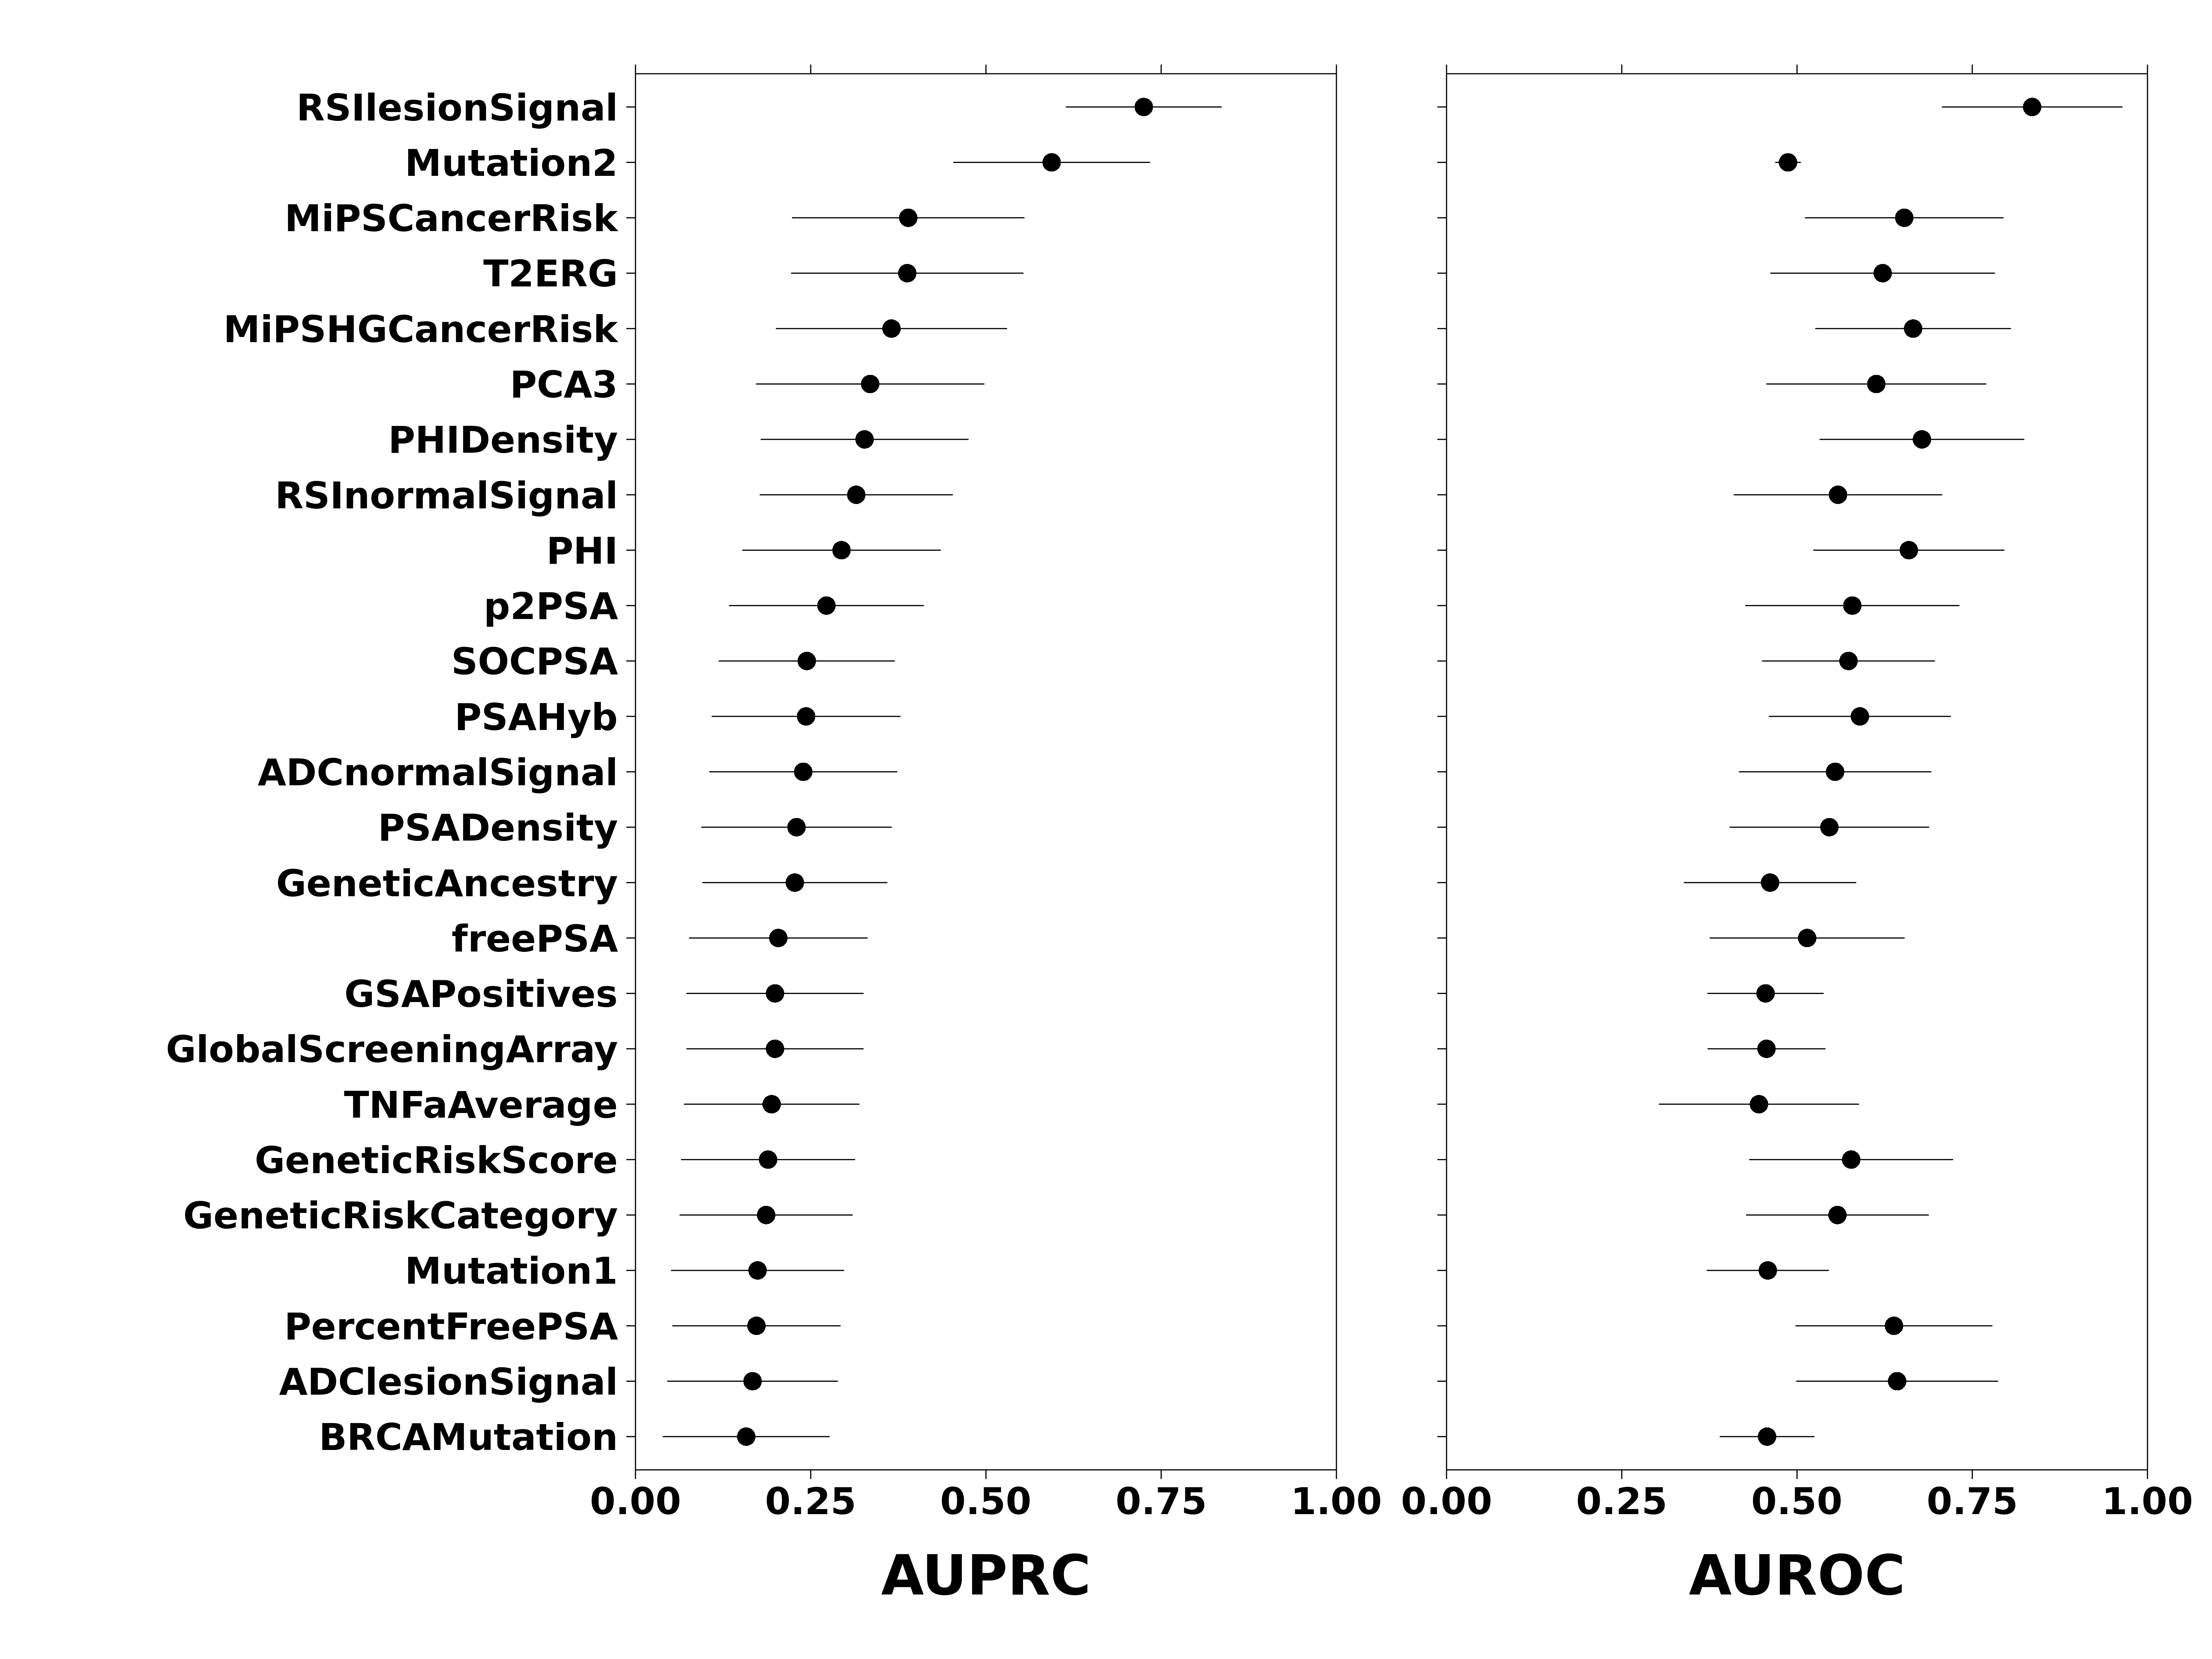
\includegraphics[keepaspectratio=false,scale=0.3]{png/auprc_auroc.png}
}
\captionof{figure}{Forest plot for AUPRC and AUROC Curves of the tests used in AS.}
\label{fig:auprc_auroc_plot}     
\end{minipage} \\

\section{Sequential Testing}

\noindent Sequential testing was performed to determine under what condition a patient that did a test A
needs to do test B. Patients on AS do a set of tests over a period of time to monitor the progression 
of their cancer. The idea behind is to find an optimal sequence of tests such that the overall sensitivity 
and specificity are maximized at lower cost, and also reduce the number of tests for the entire procedure. \\

\noindent For this sequential testing, leave-one-out cross-validation was performed in each test, their 
optimal thresholds were determined (See Methods) to build the confusion matrix, and subsequently all variables
such F$_{1}$-scores, sensitivity and specificity were reported in Table~\ref{tab:optimal}. \\

\begin{longtable}{|c|c|c|c|} 
\hline
{\bf Test } & {\bf Threshold} & {\bf Sensitivity} & {\bf Specificity} \\
\hline
      RSI lesion Signal  &  57  &  0.73 & 0.92  \\
\hline
                  PHI  &  45  &  0.58 & 0.71  \\
\hline
                p2PSA  &  13  &  0.50 & 0.58  \\
\hline
     MiPS High Grade Cancer Risk  &  30  &  0.80 & 0.55  \\
\hline
                 PCA3  &  27  &  0.73 & 0.48  \\
\hline
       MiPS Cancer Risk  &  47  &  0.87 & 0.45  \\
\hline
      RSI normal Signal  &  16  &  0.73 & 0.45  \\
\hline
      Genetic Ancestry  &   3.00  &  0.92 & 0.29  \\
\hline
               PSA Hybrid  &  4.00  &  1.00 & 0.27  \\
\hline
               SOCPSA  &   4.00  &  1.00 & 0.25  \\
\hline
      ADC normal Signal  & 829  &  1.00 & 0.23  \\
\hline
                T2ERG  &   1.00  &  0.93 & 0.21  \\
\hline
              freePSA  &   0.35  &  1.00 & 0.10  \\ 
\hline
     Genetic Risk Score  &   3.0  &  1.00 & 0.10  \\
\hline
      ADC lesion Signal  & 323  &  0.92 & 0.03  \\
\hline
       Percent Free PSA  &   6.2  &  1.00 & 0.03  \\
\hline
          TNFa Average  &   1.41  &  1.00 & 0.03  \\
\hline
         BRCA Mutation  &   0.00  &  1.00 & 0.00  \\  
\hline
  Genetic Risk Category  &   1.00  &  1.00 & 0.00  \\  
\hline
 Global Screening Array  &   0.00  &  1.00 & 0.00  \\ 
\hline
         GSA Positives  &   0.00  &  1.00 & 0.00  \\ 
\hline
            Mutation 1  &   0.00  &  1.00 & 0.00  \\ 
\hline
            Mutation 2  &   0.00  &  1.00 & 0.00  \\
\hline
\caption{Optimal threshold for each test determined by leave-one-out cross-validation}
\label{tab:optimal}
\end{longtable}

\noindent To make a sequential testing, the process can be illustrated as follows:  
A group of N subjects did test A.  Using the threshold determined by the cross-validation, 
a portion of these subjects, N-X, is classified as positive (true positive and false negative) 
and X subjects are considered negative (true negative and false positive). 
Thus, the positive cases (true and false) will go to the next test. \\

\noindent As previously mentioned, some of those tests performed to the subjects have strong correlation 
with other tests (See Figure~\ref{fig:correlations}). That will be useful to reduce the number of tests 
included in the sequential testing. Health care provider could choose a test based on pre-defined criteria such 
as specificity, cost, invasive/non-invasive, easy to administer, etc. \\

\noindent The simplest sequential testing consists of a pair of tests. Using the outputs from the cross-validation
analysis, all the tests were paired each other, and their respective overall sensitivity/specificity were 
evaluated. The top biomarkers with high sensitivity and specificity are: {\verb|RSIlesionSignal|}, {\verb|PHI|}, 
{\verb|p2PSA|}, {\verb|MiPSHGCancerRisk|}, {\verb|PCA3|}, {\verb|MiPSCancerRisk|}, and {\verb|RSInormalSignal|}. 
The results for all of the pairs of tests are shown as heatmaps in Figure~\ref{fig:pairs}. The heatmaps were 
created based on the following criteria: 1) To make a fair comparison, only subject who did all the tests 
administered in this study were considered. 2) For the overall sensitivity/specificity, 
Equations~\ref{eq:two.test.sensitivity} and ~\ref{eq:two.test.specificity} were used. \\

\begin{minipage}{\linewidth}
\makebox[\linewidth]{
  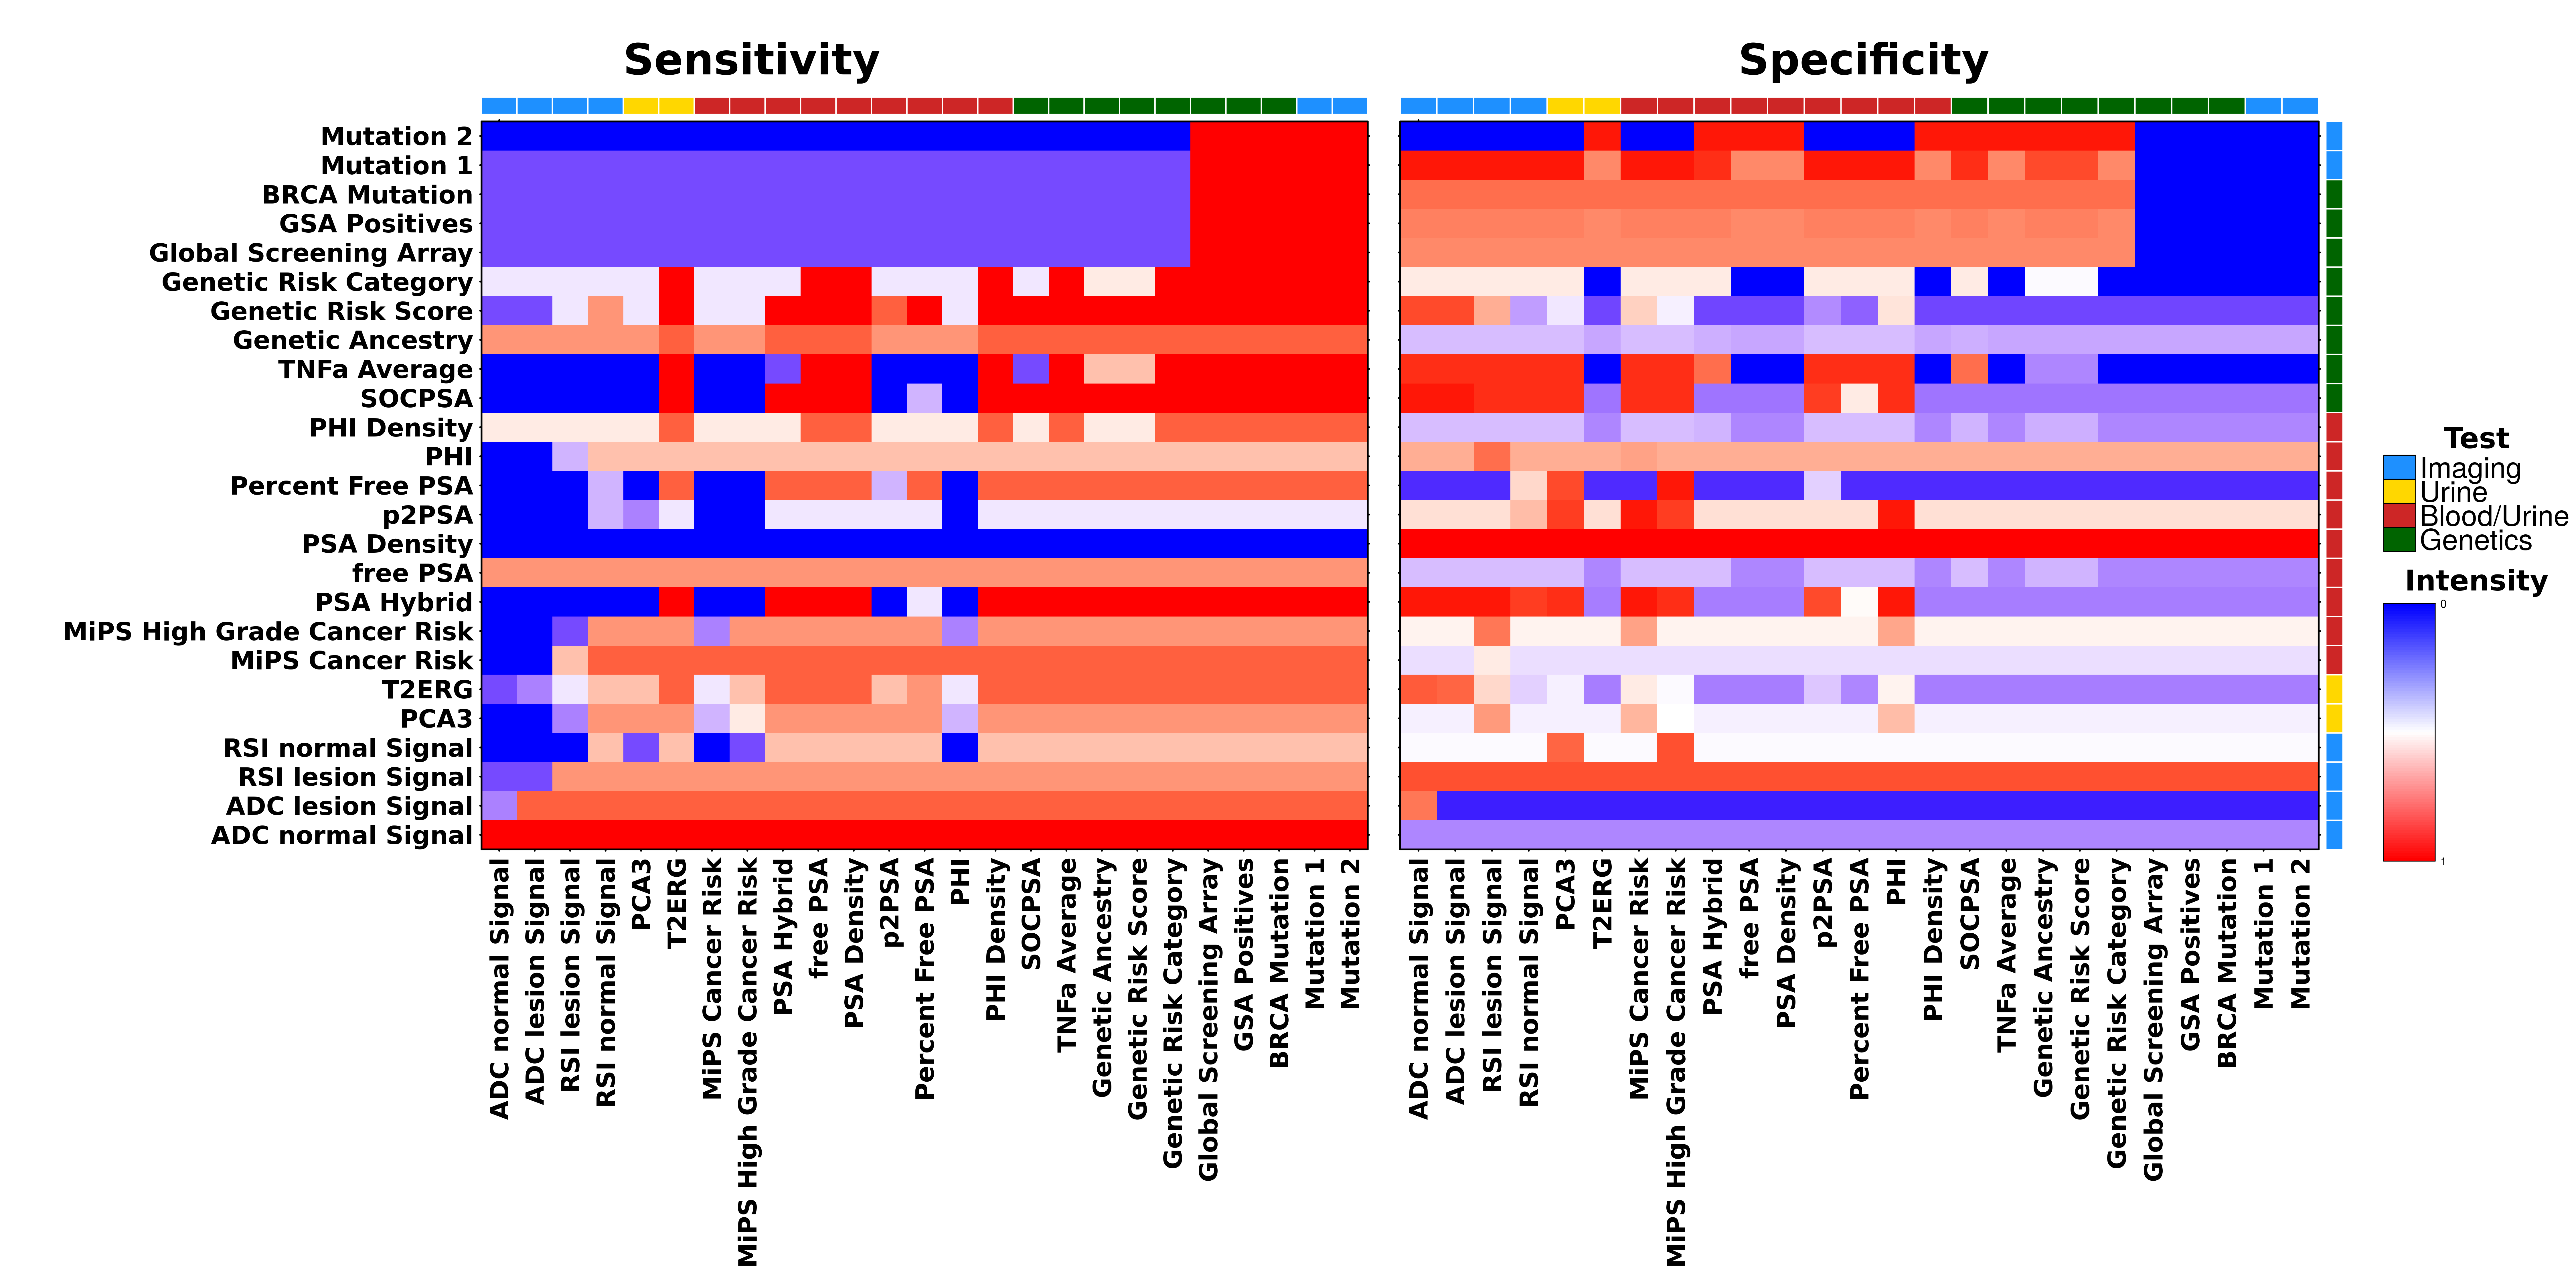
\includegraphics[keepaspectratio=true,scale=0.25]{png/pairs_sensitivity_specificity.png}
}
\captionof{figure}{Overall Sensitivity/Specificity for Pairs of Tests. Notice that the order of the tests changes the outcome}
\label{fig:pairs}
\end{minipage} \\
\\
\noindent Tests {\verb|PCA3|}, {\verb|MiPSCancerRisk|}, and {\verb|MiPSHGCancerRisk|} 
are highly correlated each other and therefore, for sequential testing purposes, one can be chosen. 
Based on the principles from sequential testing (See Methods), {\verb|MiPSHGCancerRisk|} would be the 
chosen test. Also, it is important to notice that this test is a  combination of multiple tests which includes 
\verb|PCA3|.  \\

\noindent Thus, as a first attempt to make a sequential testing could be as follows: \\

% test2 <- data.frame(predictedA=biodb$RSIlesionSignal, 
% predictedB=biodb$PHI, 
% predictedC=biodb$p2PSA, 
% predictedD=biodb$MiPSHighGradeCancerRisk)
% predictedE=biodb$RSInormalSignal)
% 
% test<- data.frame(ID=biodb$Record.ID, actual=biodb$BiopsyUpgraded)
% master<-cbind(test, test2)
% master <- master[complete.cases(master),]

% RSIlesionSignal 
%  confusion.matrix(master[,c(1,2,3)], 56.56291)
%     2  8  9 10 15 16 17 22 40 49 55 56 58 60 63
%  TP    8  9 10 15       22 40    55 56    60 63
%  FP 2             16 17       49       58  
%  tp fp fn tn
%  10  5  2 51
%  %PHI
%  confusion.matrix(master[ c(8,9,10,15,22,40,55,56,60,63) ,c(1,2,4)], 44.70000)
%  confusion.matrix(master[ c(2,16,17,49,58) ,c(1,2,4)], 44.70000)
%  TP 1  2  4  5  7  9 10
%  FP 1 4
%    tp fp fn tn
%  TP 7  0  3  0
%  FP 0  2  0  3
%  
%  
%  %p2PSA
%  confusion.matrix(master[c((8,9,15,22,55,56,63) ,c(1,2,5)], 13.21000)
%  confusion.matrix(master[c((2,49) ,c(1,2,5)], 13.21000)
%  1 2 3 5 6 7
%  tp  6  0  1  0
%  1
%  FP    0  1  0  1
%  
%  MiPSHGCancerRis
%   confusion.matrix(master[c(8,9,15,55,56,63) ,c(1,2,6)], 30.00000)
%   confusion.matrix(master[c(2) ,c(1,2,6)], 30.00000)
%  TP 6  0  0  0 
%  FP NA NA  0  1 

\begin{itemize}
  \item RSIlesionSignal 
  \item PHI 
  \item p2PSA 
  \item MiPSHGCancerRisk 
  \item RSInormalSignal 
\end{itemize}

\noindent This is a configuration above is a set of imaging/blood/urine tests. 
To visualize the sequential testing for this set, the tree in Figure~\ref{fig:tree} 
highlights the process. At the topf of the tree, the confusion matrix for \verb|RSIlesionSignal|
is computed. The positive outcomes from  \verb|RSIlesionSignal| 
(TP =10 and FP=5), will go to the next test, \verb|PHI|. It determines TP=7 and FP=2. And this  
procedure continues until the TP and TN cannnot be reduced.  At that moment, the procedure 
stops and \verb|RSINormalSignal| was not necessary to implement.  \\

\begin{minipage}{\linewidth}
\makebox[\linewidth]{
\Tree[.Subjects 
        [.Positive(RSIlesionSignal) [.FN 2  ][.TP [.10(PHI) [.FN 3 ][.TP [.7(p2PSA) [.FN 1 ] [.TP [.6(MiPSHGCancerRisk) [.FN 0 ]  [.TP 6 ]]  ]]  ] ]]]
        [.Negative(RSIlesionSignal) [.TN 51 ][.FP [.5(PHI)  [.TN 3 ][.FP [.2(p2PSA) [.TN 1 ] [.FP [.1(MiPSHGCancerRisk) [.TN 1 ]  [.FP 0 ]]  ]]  ] ]]] ]
}
\captionof{figure}{RSIlesionSignal-PHI-p2PSA-MiPSHGCancerRisk}
\label{fig:tree}
\end{minipage} \\
\\
\noindent A relevant detail is that {\verb|PHI|} test is a combination of three PSA forms: total PSA, 
free PSA, and p2PSA. In that case, this first approach could be reduced even further, and a simplified 
tree is shown in Figure~\ref{fig:tree2}. By reducing the number of tests, it helps reduce cost and 
anxiety/stress from the patient.  \\
\\
\begin{minipage}{\linewidth}
\makebox[\linewidth]{
\Tree[.Subjects 
     [.Positive(RSIlesionSignal) [.FN 2  ][.TP [.10(PHI) [.FN 3 ][.TP [.7(MiPSHGCancerRisk) [.FN 0 ] [.TP [.7 ]  ]]  ] ]]]
     [.Negative(RSIlesionSignal) [.TN 51 ][.FP [.5(PHI)  [.TN 3 ][.FP [.2(MiPSHGCancerRisk) [.TN 2 ] [.FP [.0 ]  ]]  ] ]]] ]
}
\captionof{figure}{Sequential test after removing p2PSA: RSIlesionSignal-PHI-MiPSHGCancerRisk. One step is saved with this 
sequence with better overall sensitivity.}
\label{fig:tree2}
\end{minipage} \\

\newpage

% \noindent Since we have results from a variety of tests, we can configure the sequence testing that satisfies patient needs. 
% The heatmap of the correlations in Figure~\ref{fig:correlations} is helpful for our purposes. If we want to perform a sequence 
% of tests that is comfortable and relatively easy to administer to the subjects, we could start with {\verb|PHI|} and 
% \verb|MiPSHGCancerRisk| since these tests are blood/urine type of tests and are combination of tests performed 
% in this study. \\
% 
% \noindent If we want to maximize the sensitivity and specificity of the sequential testing, we need to choose tests 
% that are not correlated each other with high sensitivity and specificity. The overall sensitivity is the product of 
% the sensitivities of the tests, and the overall specificity is an additive function.  Thus, there is a trade-off. 
% Adding more tests improves specificity with the risk to decline sensitivity, raises cost, and create 
% inconveniences to the patients.  By looking at Table~\ref{tab:optimal}, we could choose tests with 
% high sensitivity (close to 1) and perform the sequential tests.  Some of the tests in the list have very low specificity. 
% That could be a potential issue because they will not be able to filter out the false positives at the early 
% stage of the sequence. To solve it, there will be many tests to be performed and that is not the goal. 
% To illustrate this situation, we have the combination \verb|MiPSCancerRisk| - \verb|GeneticAncestry| 
% that designs a blood/urine/genetic tests set. So, the tree in Figure~\ref{fig:tree3} highlights the results. \\
% 
% \begin{figure}
% \Tree[.Subjects 
%      [.Positive(MiPSCancerRisk) [.FN 1  ][.TP [.11(GeneticAncestry) [.FN 1 ][.TP [.10  ]  ] ]]]
%      [.Negative(MiPSCancerRisk) [.TN 26 ][.FP [.33(GeneticAncestry) [.TN 8 ][.FP [.25  ]  ] ]]] ] 
% \caption{Sequential test MiPSCancerRisk - GeneticAncestry}
% \label{fig:tree3}
% \end{figure}
% 
% 
% \begin{figure}
% \Tree[.Subjects 
%      [.Positive(GeneticAncestry) [.FN 1  ][.TP [.11(MiPSCancerRisk) [.FN 1 ][.TP [.10  ]  ] ]]]
%      [.Negative(GeneticAncestry) [.TN 17 ][.FP [.42(MiPSCancerRisk) [.TN 17 ][.FP [.25  ]  ] ]]] ] 
% \caption{Sequential test GeneticAncestry - MiPSCancerRisk}
% \label{fig:tree4}
% \end{figure}

% \section{Pairing Tests}
% 
% \noindent A more formal way to perform this sequential testing is to try out all possibilities 
% from the tests used in this study. The simplest way is to make pairs of tests. 
% We want to find sequential tests that maximize sensitivity/specificity. 
% In Figure~\ref{fig:pairs}, we paired all the tests in this study and we determine 
% the overall sensitivity/specificity. \\
% 
% \noindent The heatmaps were created based on these criteria: 1) To make a fair comparison, 
% we considered all subject who did all the tests administered in this study. 
% 2) For the overall sensitivity/specificity, Equations~\ref{eq:two.test.sensitivity} and 
% ~\ref{eq:two.test.specificity} are used. \\

% \noindent Both overall sensitivity/specificity can help to 
% identify tests with high sensitivity/specificity. From Figure~\ref{fig:pairs}, 
% these tests are potential candidates for sequential testings:  {\verb|RSIlesionSignal|} , 
% {\verb|PHI|},  {\verb|MiPSHGCancerRisk|},  {\verb|MiPSHGCancerRisk|},  
% {\verb|PCA3|}, {\verb|MiPSCancerRisk|}, and  {\verb|RSInormalSignal|}.  Using this procedure we can
% explore other designs of sequential testing. \\

\section{Survival Analysis}

\noindent In this section, survival analysis was performed. From the original data, the time field
\verb|DaysDxToUpgrade| was initially considered. It contains data from patients whose \verb|BiopsyUpgraded|
have a value of 1. The remaining empty rows (patients with \verb|BiopsyUpgraded| equals to 0) were replaced
with \verb|DaysBxToLastReview|. Considering the top biomarkers used described in the previous section, 
the Kaplan-Meier survival plots are shown below: \\

\begin{minipage}{\linewidth}
\makebox[\linewidth]{ 
  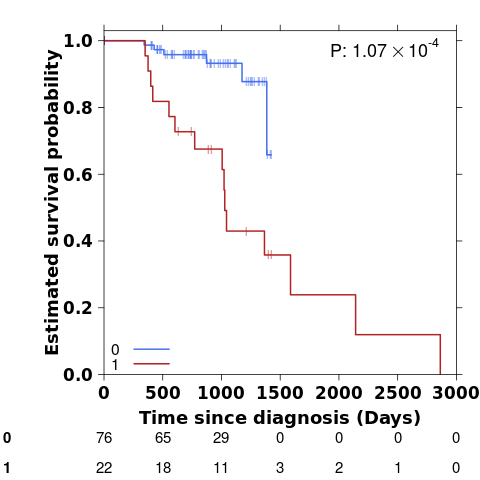
\includegraphics[keepaspectratio=true,scale=0.6]{png/Kaplan_Meier_RSIlesionSignal.png}
}
\captionof{figure}{Kaplan-Meier Plot for RSI lesion Signal}
\label{fig:KM_PHI}
\end{minipage} \\


\begin{minipage}{\linewidth}
\makebox[\linewidth]{
  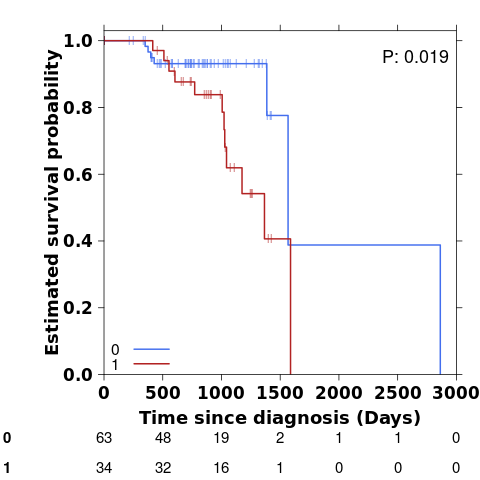
\includegraphics[keepaspectratio=true,scale=0.6]{png/Kaplan_Meier_PHI.png}
}
\captionof{figure}{Kaplan-Meier Plot for PHI}
\label{fig:KM_PHI}
\end{minipage} \\


\begin{minipage}{\linewidth}
\makebox[\linewidth]{
  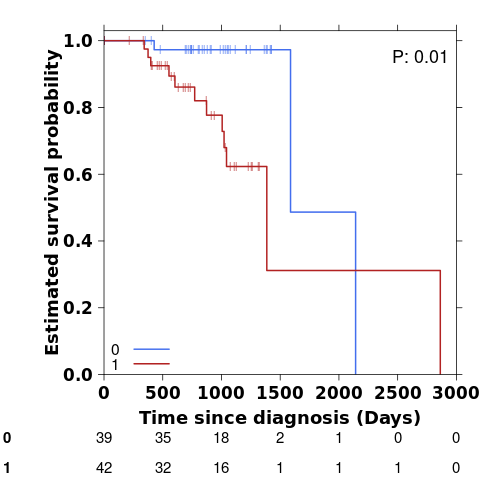
\includegraphics[keepaspectratio=true,scale=0.6]{png/Kaplan_Meier_MiPSHGCancerRisk.png}
}
\captionof{figure}{Kaplan-Meier Plot for MiPS High Grade Cancer Risk}
\label{fig:KM_MIPS}
\end{minipage} \\


%test2 <- data.frame(predictedA=biodb$MiPSCancerRisk, 
%predictedB=biodb$GeneticAncestry) 
%%predictedC=biodb$p2PSA, 
%%predictedD=biodb$MiPSHighGradeCancerRisk, 
%%predictedE=biodb$RSInormalSignal)
%
%test<- data.frame(ID=biodb$Record.ID, actual=biodb$BiopsyUpgraded)
%master<-cbind(test, test2)
%master <- master[complete.cases(master),]
%  
%   confusion.matrix(master[,c(1,2,3)], 47.00000)
%  
%  
%  
%  >  confusion.matrix(master[,c(1,2,3)], 47.00000)
%   [1]  3  4  6  7  8  9 10 11 12 14 15 16 17 18 21 22 26 27 29 31 32 33 35 37 40 44 47 49 50 53 54 56 57 58 59 60 62 63 64 66 67 68 69 71
%  tp                8  9 10          15             22          31    35       40                   56 57                64
%  fp    3  4  6  7  11 12 14  16 17 18 21  26 27 29  32 33  37 44 47 49 50 53 54  58 59 60 62 63  66 67 68 69 71
%  
%  
%    tp fp fn tn  f1.score threshold                 tp.positive.list
%  1 11 33  1 26 0.3928571        47 48,54,59,62,64,66,69,70,76,93,94
%  
%  Genetic Ancestry
%  >  confusion.matrix(master[  c(8,9,10,15,22,31,35,40,56,57,64) ,c(1,2,4)], 3.00000)
%   [1]  1  2  3  4  5  6  7  9 10 11
%   [1]  1  2  3  4  5  6  7  9 10 11
%    tp fp fn tn f1.score threshold    tp.positive.list
%  1 10  0  1  0 0.952381         3 1,1,1,1,1,1,1,1,4,4
%  
%  >  confusion.matrix(master[  c(3,4,6,7,11,12,14,16,17,18,21,26,27,29,32,33,37,44,47,49,50,53,54,58,59,60,62,63,66,67,68,69,71) ,c(1,2,4)], 3.00000)
%   [1]  1  2  3  4  6  7  8 10 13 14 15 16 17 19 21 22 23 24 25 26 28 29 31 32 33
%  integer(0)
%    tp fp fn tn f1.score threshold tp.positive.list tp.positive.patients
%  1  0 25  0  8        0         3         

% 
% [1]  1  2  3  4  6  7  8  9 10 12 14 15 16 18 19 20 22 23 24 27 29 31 32 33 35  36 37 38 39 41 42 46 47 48 50 51 52 53 54 55 56 57 58 59 60 61 63 64 66 68  69 70 71
% [1]                    8  9 10       15             22             31       35                                               56 57          61    64
%      1  2  3  4  6  7          12 14    16 18 19 20    23 24 27 29    32 33     36 37 38 39 41 42 46 47 48 50 51 52 53 54 55       58 59 60    63    66 68  69 70 71
% 
% confusion.matrix(master[,c(1,2,4)], 3.00000)
% 
%  tp fp fn tn  f1.score threshold      tp.positive.list
% 1 11 42  1 17 0.3384615         3 1,1,1,1,1,1,1,1,1,4,4
%                              
%  confusion.matrix(master[ c(8,9,10,15,22,31,35,  56,57,61,64)  ,c(1,2,3)], 47.00000)
% tp fp fn tn f1.score threshold              tp.positive.list
% 1 10  0  1  0 0.952381        47 54,59,62,64,66,69,7
% 
%  tp fp fn tn f1.score threshold tp.positive.list tp.positive.patients
% 1  0 25  0 17       

% \newpage
% 
% \section{Summary}
% \noindent In this study, a group of subjects went in AS and a series of tests were performed. 
% These tests were classified by types: Urine, Blood, Blood/Urine, Imaging and Genetics.  
% Many of those tests are correlated with other tests, and some of those tests 
% were combinations of simpler tests.  From the data collected in the subjects, the confusion 
% matrix for each test were determined and the ROC and Precision-Recall curves were drawn. 
% To determine the optimal threshold for each test, leave-one-out cross-validation was performed. 
% The optimal threshold was determined based on the maximum value in F$_{1}$-score. Using that 
% information, the optimal confusion matrix was determined as well as the sensitivity/specificity 
% for each test. \\

\section{Next Steps}

\noindent Systematic descriptive analysis of cohorts. \\   

\section{Methods}

\subsection{Precision-Recall (PR) Curves}

\noindent Recall or Sensitivity is the ability of the test to correctly mark all positive responses 
as positive. Precision is the ability of the test not to wrongly label a negative sample as positive. 
To make the PR curve of a test, the confusion matrix is computed based on the scores of the test 
and the gold standard data (in this study, \verb|BiopsyUpgraded|). Each point of the PR curve (Recall, Precision)
comes from a confusion matrix at a given threshold. The threshold is applied to the scores of the test to determine
which scores are predicted as positive (1) and negative (0). Using these predicted values, the elements of the 
confusion matrix are computed and other variables such as accuracy, precision, sensitivity and specificity, 
F$_{1}$-score can be easily obtained. The area under the Precision-Recall curve (AUPRC) can be computed using 
the trapezoid rule. A similar procedure is employed to make the ROC curve. \\

\subsection{Leave-One-Out Cross-Validation}

\noindent Leave-One-Out Cross-Validation is a method that trains a model by taking one point out of the dataset 
as a test data and the remaining points are used to train the model. Once the optimal model is found, 
the model is evaluated using the test data. And this process is done repetively such that all points 
will be used as test data. In this study, the model is the confusion matrix with the optimal threshold.
The criterion to determine that threshold is based on F$_{1}$-score.  \\

\subsection{Sequential Tests}

\noindent Serial or sequential testing is useful in some clinical situations to potentially avoid 
the need for a subsequent test. For the case of two tests, A and B, the computation of the sensitivity 
and specificity are given by: \\

\begin{equation}
  \mbox{Sensitivity(A,B)}  = \mbox{Sensitivity}_{A} . \mbox{Sensitivity}_{B}
\label{eq:two.test.sensitivity}
\end{equation}

\begin{equation}
  \mbox{Specificity(A,B)} =  \mbox{Specificity}_{A} + [1 - \mbox{Specificity}_{A}] . \mbox{Specificity}_{B}
\label{eq:two.test.specificity}
\end{equation}

\noindent From these equations, it is clear that more tests performed, overall sensitivity will decline 
and overall specificity will increase. Sequential testing looks for an increase in the positive 
predictive value, {\it i.e} , determine that a subject with a condition truly has the condition. 
Thus, in each stage the test has to report positive. Otherwise, the procedure stops.  \\

\noindent Based on Equation~\ref{eq:two.test.specificity}, a good guess to make a sequential testing is to choose
a test with a high sensitivity. That makes the first term dominant. The reason behind to choose a test by 
specificity is that the test with high specificity will reduce the group of subjects to go to the next test 
by excluding the negative cases from the group. This can be seen from the specificity formula: $tn/(tn+fp)$.
The maximum value is reached when $fp=0$. Thus, the list of positive subjects to go to the next test will be smaller. \\ 

\section{Appendix}

\noindent Current spreadsheet (04/20/2020) has the following columns: \\

\begin{longtable}{| p{.40\textwidth} | p{.60\textwidth} |} 
\hline
{\bf Column Name} & {\bf Description}  \\
\hline
BiopsyUpgraded           &    Research study biopsy increased cancer grade from most recent previous biopsy result \\
\hline
PCA3                     &    Urinary biomarker \\
\hline
T2ERG                    &    Urinary biomarker \\
\hline
MiPSCancerRisk           &    Urinary/Blood biomarker using PSA, PCA3, T2ERG (Mi-Prostate Score Cancer Risk) \\
\hline
MiPSHighGradeCancerRisk  &    Urinary/Blood biomarker using PSA, PCA3, T2ERG (Mi-Prostate Score High Grade Cancer Risk, Gleason Score ≥7) \\
\hline
PSAHyb                   &    Blood biomarker (Access Hybritech PSA assay) \\
\hline
freePSA                  &    Blood biomarker (amount of unbound PSA) \\
\hline
p2PSA                    &    Blood biomarker ([-2]proPSA, precursor of PSA) \\
\hline
PercentFreePSA           &    Blood biomarker (percentage of unbound PSA) \\
\hline
PHI                      &    Blood biomarker (Prostate Health Index) \\
\hline
GeneticAncestry          &    Genetic biomarker (Scores: 1:European, 2:African, 3:East Asian, 4:Native American) \\
\hline
GeneticRiskScore         &    Genetic biomarker (Scores: 1:Low, 2:Normal, 3:High) \\
\hline
GeneticRiskCategory      &    Genetic biomarker (Scores: 1, 2 and 3) \\
\hline
GlobalScreeningArray     &    Genetic biomarker (Scores: 0 and 1) \\
\hline
GSAPositives             &    Genetic biomarker (Scores: 0 and 1) \\
\hline
BRCAMutation             &    Genetic biomarker (BRCA1 or BRCA2 gene mutation) (0: Negative, 1:Positive) \\
\hline
Mutation1                &    Genetic biomarker (if Global Screening Array positive:  0:Negative 1:BRCA1, 2:BRCA2, 3:ATM, 4:MLH1, 5:PMS2  )  \\
\hline
Mutation 2               &    Genetic biomarker (if Global Screening Array positive:  0:Negative 1:BRCA1, 2:BRCA2, 3:ATM, 4:MLH1, 5:PMS2  )  \\
\hline
RSInormalSignal          &    Imaging biomarker (Continuous values) \\
\hline
RSIlesionSignal          &    Imaging biomarker (Continuous values) \\
\hline
ADCnormalSignal          &    Imaging biomarker (Continuous values) \\
\hline
ADClesionSignal          &    Imaging biomarker (Continuous values) \\
\hline
TNF average              & \\
\hline                   
SOCPSA                   & \\
\hline
\caption{Test used fo this study}
\label{tab:info}
\end{longtable}

\begin{thebibliography}{}
\bibitem{JAMES}
  James, G.~{\textit{et al.}}. An Introduction to Statistical Learning. Springer. 7th Printing.
\bibitem{BPG}
C.~P'ng.~{\textit{et al.}}. BPG: Seamless, Automated and Interactive Visualization of Scientific Data.
\textit{BMC Bioinformatics} 20, 42 (2019).\\

\end{thebibliography}

\end{document}
